%% REGISTRY: Theorem n | Lemma n | source | eq. numbers
%%  Thm 1  BSM price of a European call | Lesson 3, cells 37, 48  | eq:call, eq:d1d2
%%  Thm 2  Greeks of the European call  | Lesson 3, cells 46-49   | eq:callgreeks
%%  Thm 3  Put-call parity              | Lesson 3, cell 30       | eq:parity
%%  Lem 1  BSM price of a European put  | from Thm 1, Thm 3       | eq:put
\RequirePackage{fix-cm}
\documentclass[11pt,a4paper]{article}
\usepackage[utf8]{inputenc}
\usepackage[margin=2cm]{geometry}
\usepackage{amsmath,amssymb,mathtools}
\usepackage{graphicx}
\usepackage{booktabs,array}
\usepackage[most]{tcolorbox}
\usepackage{enumitem}
\setlist[itemize]{itemsep=1pt, topsep=2pt, label=$\bullet$}
\setlist[enumerate]{itemsep=1pt, topsep=2pt}
\usepackage{listings}
\usepackage{tikz}
\usepackage{pgfplots}
\pgfplotsset{compat=1.18}
\usetikzlibrary{arrows.meta,positioning,shapes.geometric,calc}
% ---- matplotlib look for the plots drawn by LaTeX (no image files needed)
\definecolor{tabblue}{HTML}{1F77B4}\definecolor{taborange}{HTML}{FF7F0E}
\definecolor{tabgreen}{HTML}{2CA02C}\definecolor{tabred}{HTML}{D62728}
\pgfplotsset{mpl/.style={scale only axis, axis line style={black,line width=0.8pt},
  tick style={black,line width=0.8pt}, tick align=outside, xtick pos=bottom, ytick pos=left,
  major tick length=3.5pt, tick label style={font=\fontsize{10}{12}\selectfont\sffamily},
  legend cell align=left, legend style={draw=black!20, rounded corners=2pt, fill=white, fill opacity=0.8, text opacity=1},
  legend image code/.code={\draw[#1] (0pt,0pt) -- (22pt,0pt);}},
  mplgrid/.style={grid=major, major grid style={black!30, line width=0.8pt, dash pattern=on 2.96pt off 1.28pt}}}
\tikzset{mpldash/.style={dash pattern=on 3.7pt off 1.6pt}, mpldot/.style={dash pattern=on 1pt off 1.65pt}}
\usepackage{caption}
\usepackage{hyperref}
\hypersetup{colorlinks=true,linkcolor=black,citecolor=black,urlcolor=black,
  pdftitle={Financial Processes -- Homework of Lesson 3 (HW 2/1--2/4), short version},pdfauthor={Carlos Chipantiza}}
\usepackage{needspace}
\frenchspacing

\definecolor{DefBlue}{RGB}{16,64,120}
\definecolor{LemRed}{RGB}{170,30,40}
\definecolor{ThmPurple}{RGB}{95,40,130}
\definecolor{Hl}{RGB}{255,242,160}
\definecolor{AnsGreen}{RGB}{20,120,70}
\definecolor{CodeGray}{RGB}{110,110,110}
\definecolor{Flow}{RGB}{16,64,120}
\definecolor{HC}{RGB}{230,140,20}
\definecolor{BUG}{RGB}{190,30,40}
\definecolor{FIX}{RGB}{20,120,70}

\newcounter{defn}\newcounter{lemn}\newcounter{thmn}
\newtcolorbox{defbox}[1]{enhanced,colback=white,colframe=DefBlue,boxrule=0.8pt,arc=1mm,left=2mm,right=2mm,top=1.5mm,bottom=1.5mm,
  before upper={\refstepcounter{defn}\noindent\textbf{Definition \thedefn} (#1).\par\smallskip}}
\newtcolorbox{lembox}[1]{enhanced,colback=white,colframe=LemRed,boxrule=0.8pt,arc=1mm,left=2mm,right=2mm,top=1.5mm,bottom=1.5mm,
  before upper={\refstepcounter{lemn}\noindent\textbf{Lemma \thelemn} (#1).\par\smallskip}}
\newtcolorbox{thmbox}[1]{enhanced,colback=white,colframe=ThmPurple,boxrule=0.8pt,arc=1mm,left=2mm,right=2mm,top=1.5mm,bottom=1.5mm,
  before upper={\refstepcounter{thmn}\noindent\textbf{Theorem \thethmn} (#1).\par\smallskip}}
\newtcolorbox{ansboxenv}{enhanced,colback=AnsGreen!6,colframe=AnsGreen,boxrule=0.8pt,arc=1mm,left=2mm,right=2mm,top=1.5mm,bottom=1.5mm}
\newcommand{\ansbox}[1]{\begin{ansboxenv}#1\end{ansboxenv}}
\newenvironment{exercise}[1]{\par\medskip\noindent\textbf{#1.}\ }{\par\medskip}
\newcommand{\solution}{\par\noindent\textbf{\textit{Solution.}}\ }
\newcommand{\hl}[1]{\colorbox{Hl}{#1}}
\newcommand{\case}[1]{\par\smallskip\noindent\hl{#1}\ }

% ---- code that can be copied from the PDF and pasted into Python:
% every space is a real character (an invisible glyph mapped to U+0020), no line
% numbers, no line breaks inside a line, straight quotes.
\input{glyphtounicode}
\pdfglyphtounicode{visiblespace}{0020}
\pdfgentounicode=1
\makeatletter
\def\lst@visiblespace{{\color{white}\char32}}
\makeatother
\lstdefinestyle{py}{language=Python,basicstyle=\ttfamily\footnotesize,keywordstyle=\color{DefBlue},
  commentstyle=\color{CodeGray},stringstyle=\color{black},showspaces=true,showstringspaces=false,
  frame=single,rulecolor=\color{CodeGray},numbers=none,
  breaklines=false,columns=fixed,basewidth=0.5em,keepspaces=true,tabsize=4,xleftmargin=0.4em,framexleftmargin=0.4em,
  captionpos=t,literate={\$}{{\char36}}1 {'}{{\char13}}1 {`}{{\char18}}1}
\lstdefinestyle{prof}{style=py,basicstyle=\ttfamily\fontsize{7.2}{8.4}\selectfont}
\lstdefinestyle{out}{basicstyle=\ttfamily\footnotesize,columns=fixed,basewidth=0.5em,showspaces=true,
  frame=leftline,framerule=1.2pt,rulecolor=\color{FIX},numbers=none,xleftmargin=0.8em,framexleftmargin=0.4em,
  breaklines=false,captionpos=t}
\captionsetup[lstlisting]{labelformat=empty,font={footnotesize,sf},justification=raggedright,singlelinecheck=false,skip=2pt}
\newcommand{\src}[2]{\texttt{#1}, lines #2}
\renewcommand{\lstlistingname}{Code}
\newcommand{\subhead}[1]{\par\medskip\noindent{\large\bfseries #1}\par\smallskip\noindent\ignorespaces}
% everything is inside this file: the code is written here and the plots are drawn by pgfplots
\newcommand{\PP}{\mathbb{P}}
% ---- flowcharts (HW 2/1)
\tikzset{
  fbase/.style={draw=Flow,line width=0.7pt,align=center,font=\footnotesize,minimum height=7mm,text width=74mm,inner sep=2.5pt},
  fterm/.style={fbase,rounded corners=3.5mm,fill=Flow!10},
  fproc/.style={fbase,rectangle},
  fhc/.style={fbase,rectangle,fill=HC!22,draw=HC!80!black},
  fnew/.style={fbase,rectangle,fill=FIX!10,draw=FIX!80!black},
  fdec/.style={fbase,diamond,aspect=3.4,text width=42mm,inner sep=0.5pt,fill=Flow!4},
  ferr/.style={fbase,rectangle,draw=BUG,fill=BUG!8,text width=32mm},
  farr/.style={-{Stealth[length=2.2mm]},line width=0.6pt,draw=Flow},
  tagH/.style={circle,fill=HC!85!black,text=white,font=\scriptsize\bfseries,inner sep=1pt,minimum size=5mm},
  tagB/.style={circle,fill=BUG,text=white,font=\scriptsize\bfseries,inner sep=1pt,minimum size=5mm},
  tagF/.style={circle,fill=FIX,text=white,font=\scriptsize\bfseries,inner sep=1pt,minimum size=5mm},
  flab/.style={font=\scriptsize,text=Flow}
}
\DeclareRobustCommand{\tH}[1]{\tikz[baseline=-0.6ex]\node[tagH,minimum size=4mm,inner sep=0pt,font=\tiny\bfseries]{H#1};}
\DeclareRobustCommand{\tB}[1]{\tikz[baseline=-0.6ex]\node[tagB,minimum size=4mm,inner sep=0pt,font=\tiny\bfseries]{B#1};}
\DeclareRobustCommand{\tF}[1]{\tikz[baseline=-0.6ex]\node[tagF,minimum size=4mm,inner sep=0pt,font=\tiny\bfseries]{#1};}
\newcommand{\sq}{\char13}
\newcommand{\lb}{\char`\{}
\newcommand{\rb}{\char`\}}
\newcommand{\dd}{\,\mathrm{d}}

\begin{document}
\noindent Name: Carlos Chipantiza \hfill Neptun code: EACN90\\
\noindent Financial Processes (BMETE95MM14), BME, Fall 2026\\[2pt]
{\large\textbf{Homework of Lesson 3: HW 2/1 -- HW 2/4}}\\[2pt]
\noindent\rule{\textwidth}{0.4pt}

\noindent\textbf{Remark.} The results used are stated in boxes before the exercise where they are first needed and are cited by number together with the displayed equation; each one is a result of Lesson~3 (2026 notebook; the cell is given in the box), or it is proved right after its box. The code of HW 2/1 is in \texttt{plotter.py} and \texttt{hw21\_examples.py}; the code of HW 2/2--2/4 is in the notebooks \texttt{1\_HW\_EXE\_2}, \texttt{1\_HW\_EXE\_3} and \texttt{1\_HW\_EXE\_4}, in the same order as here. In the new versions, each change is marked \texttt{\# change \# k} \dots\ \texttt{\# end change \# k}, and a replaced line of the professor's code is kept as a \texttt{\#Delete.} comment. All code shown can be copied from this PDF and pasted into Python (spaces and indentation are kept; there are no line numbers).

% ============================================================================ HW 2/1
\begin{exercise}{HW 2/1}
Smart up our plotter to be able to customize the hard-coded layout setup inside the function. Add more custom feature that you would like to use.
\end{exercise}
\solution
We need to do: 
\begin{itemize}
	\item [(1)] Every layout setting that is written inside the body of the plotter of cell 9 must become a choice of the caller; 
	\item [(2)] New options of our own.
\end{itemize}



\subhead{What the plotter of cell 9 does.}
\emph{The professor's code.} Cell 9 of the 2026 notebook, verbatim (one long comment is split over two lines):
\par\smallskip\noindent\begin{minipage}{\linewidth}\begin{lstlisting}[style=prof,title={\src{professor\_cell09.py}{4--50}}]
import matplotlib.pyplot as plt
from matplotlib import rcParams # detailed parameter setting
""" more details on customization: https://matplotlib.org/stable/tutorials/introductory/customizing.html """
from typing import Dict, List, Union


# some type hints in the header of the function
def my_plotter(x: List[float], y: Union[List[float], List[List[float]]], layout: Dict = {}, names: List[str] = None) -> None:
    """ inline for loop is called 'list comprehension' """
    y = [y] if all(isinstance(item, float) for item in y) else y
    
    plt.figure(figsize=(8, 4))
    lines = []
    show_legend = True if names is not None else False
    # show_legend = True if names else False  -> here is fine, but be cautious bc 0, empty str and empty list
    # will be evaulated to False

    """ setup some basic key-word arguments for plot line """
    plot_kwargs = {
        'linestyle': 'solid',
        'linewidth': 4
    }
    if names is not None:
        show_legend = True
        if len(names) != len(y):
            raise ValueError("Length of names is not matching with number of plotted y lists.")

    """ 'enumerate' add a counter to the loop """
    for i, y_item in enumerate(y):
        if show_legend:
            plot_kwargs['label'] = names[i]
        _line = plt.plot(x, y_item, **plot_kwargs)
        lines.append(_line)

    if show_legend:
        plt.legend(fontsize=16)
    if 'title' in layout:
        plt.title(layout['title'], fontsize=20)
        rcParams['axes.titlepad'] = 30 # moving the title a little further away from the plot
    if 'x_label' in layout:
        plt.xlabel(layout['x_label'], fontsize=16)
        rcParams['axes.labelpad'] = 20 # moving the ax label a little further away from the plot

    """ enhance axes """
    ax = plt.gca() # gca: get current axes
    ax.axhline(linestyle='--', color='black', linewidth=1)
    plt.show()
\end{lstlisting}\end{minipage}\par\smallskip
Cells 10 and 11 of the notebook use it to plot the payoffs of a long and a short forward with $K=100$ (the call of cell 11 is split over several lines):
\par\smallskip\noindent\begin{minipage}{\linewidth}\begin{lstlisting}[style=py,title={\src{hw21\_examples.py}{12--27} (block 1)}]
import numpy as np

strike = 100
step_size = 0.001

x_stock_price = np.arange(0, 2 * strike, step_size)
y_forward_payoff = np.array([x - strike for x in x_stock_price])

y_forward_payoff__short = y_forward_payoff * (-1)
y_forward_payoff__short

layout = {'title': 'Forward', 'x_label': '$S_{T}$'}
my_plotter(x_stock_price, [y_forward_payoff, y_forward_payoff__short],
           layout=layout,
           names=['Long Forward Payoff at time $T$',
                  'Short Forward Payoff at time $T$'])
\end{lstlisting}\end{minipage}\par\smallskip
\emph{What it shows.} The last line of cell 10 shows the array of short-forward payoffs (with NumPy 2.2, the version of the course environment; older versions omit the second line), and cell 11 shows Figure~\ref{fig:cell9out}:
\par\smallskip\noindent\begin{minipage}{\linewidth}\begin{lstlisting}[style=out,title={output of cell 10}]
array([100.   ,  99.999,  99.998, ..., -99.997, -99.998, -99.999],
      shape=(200000,))
\end{lstlisting}\end{minipage}\par\smallskip
\begin{figure}[!ht]
\centering
\resizebox{0.62\textwidth}{!}{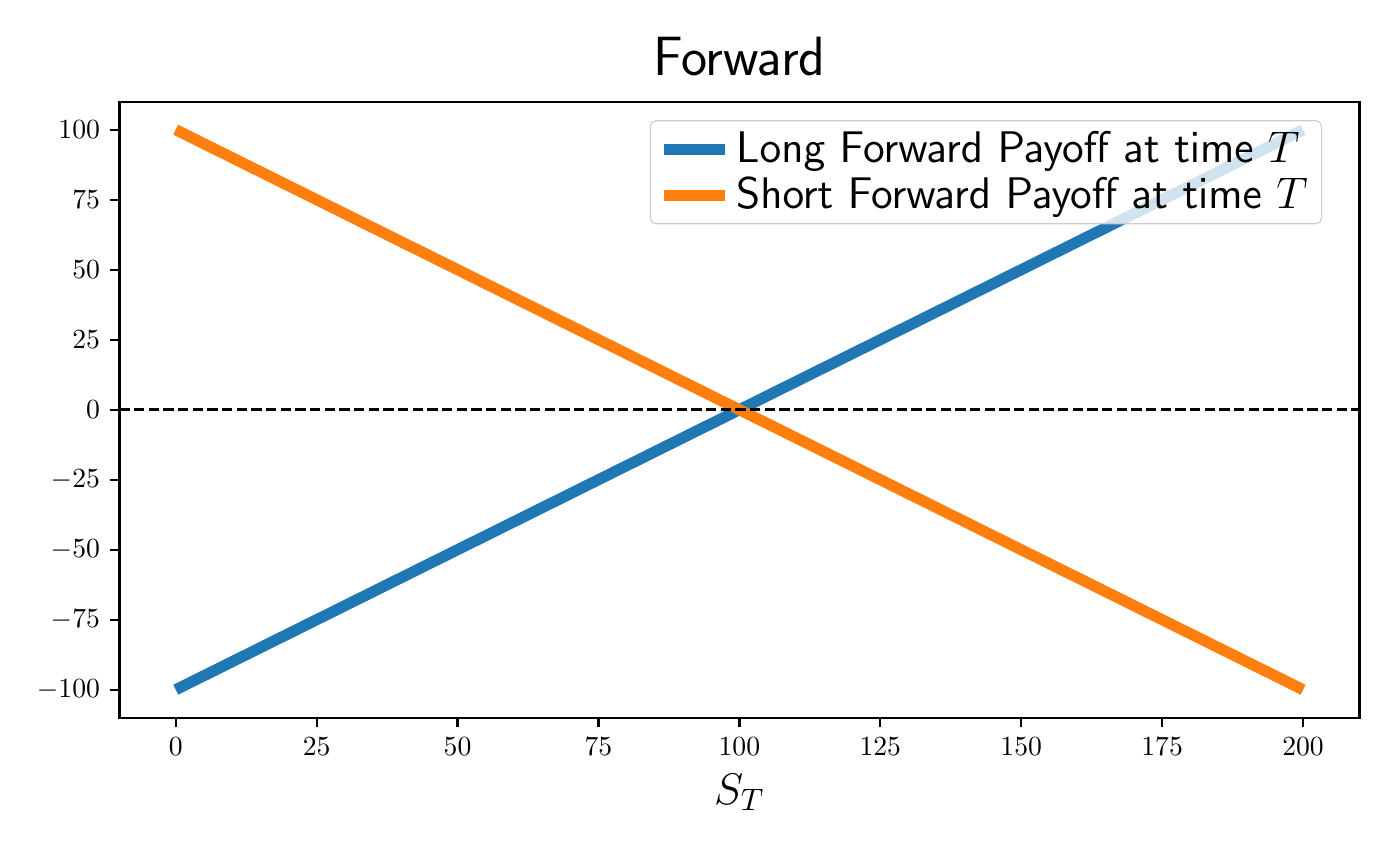
\begin{tikzpicture}
\begin{axis}[mpl, width=6.2in, height=3.08in, xmin=-10, xmax=210, ymin=-110, ymax=110,
  xtick={0,25,...,200}, ytick={-100,-75,...,100},
  title={\fontsize{20}{24}\selectfont\sffamily Forward}, title style={yshift=0pt},
  xlabel={\fontsize{16}{19}\selectfont $S_{T}$}, xlabel style={yshift=0pt},
  legend pos=north east, legend style={font=\fontsize{16}{19}\selectfont\sffamily}]
\addplot[tabblue, line width=4pt] coordinates {(0,-100) (199.999,99.999)};
\addlegendentry{Long Forward Payoff at time $T$}
\addplot[taborange, line width=4pt] coordinates {(0,100) (199.999,-99.999)};
\addlegendentry{Short Forward Payoff at time $T$}
\draw[black, line width=1pt, mpldash] (axis cs:-10,0) -- (axis cs:210,0);
\end{axis}
\end{tikzpicture}}
\caption{Output of cell 11 (block 1) in a new session: the plot drawn by the plotter of cell 9, as the notebook displays it. It is the same picture as the output stored in the course notebook.}
\label{fig:cell9out}
\end{figure}

\emph{Step by step.} Figure~\ref{fig:flow9} follows the code of cell 9 step by step. The orange boxes contain the hard-coded layout (Table~\ref{tab:hc}); of the dictionary \texttt{layout} only the keys \texttt{"title"} and \texttt{"x\_label"} are read.
\begin{center}\small
\captionof{table}{Hard-coded layout of cell 9 (orange tags of Figure~\ref{fig:flow9}).}\label{tab:hc}
\begin{tabular}{@{}clp{0.45\textwidth}@{}}
\toprule
tag & hard-coded value in cell 9 & what the caller cannot change\\
\midrule
\tH{1} & \texttt{figsize=(8, 4)} & size of the figure\\
\tH{2} & \texttt{linestyle=\sq solid\sq}, \texttt{linewidth=4} & style and width of the curves (also no colour, marker or opacity)\\
\tH{3} & \texttt{plt.legend(fontsize=16)} & legend font size (and its position)\\
\tH{4} & \texttt{fontsize=20}, \texttt{axes.titlepad = 30} & title size and its distance to the axes\\
\tH{5} & \texttt{fontsize=16}, \texttt{axes.labelpad = 20} & $x$-label size and distance (there is no $y$-label)\\
\tH{6} & dashed black line at $y=0$, width $1$ & whether this line is drawn, and where\\
\bottomrule
\end{tabular}
\end{center}


\begin{figure}[p]
\centering
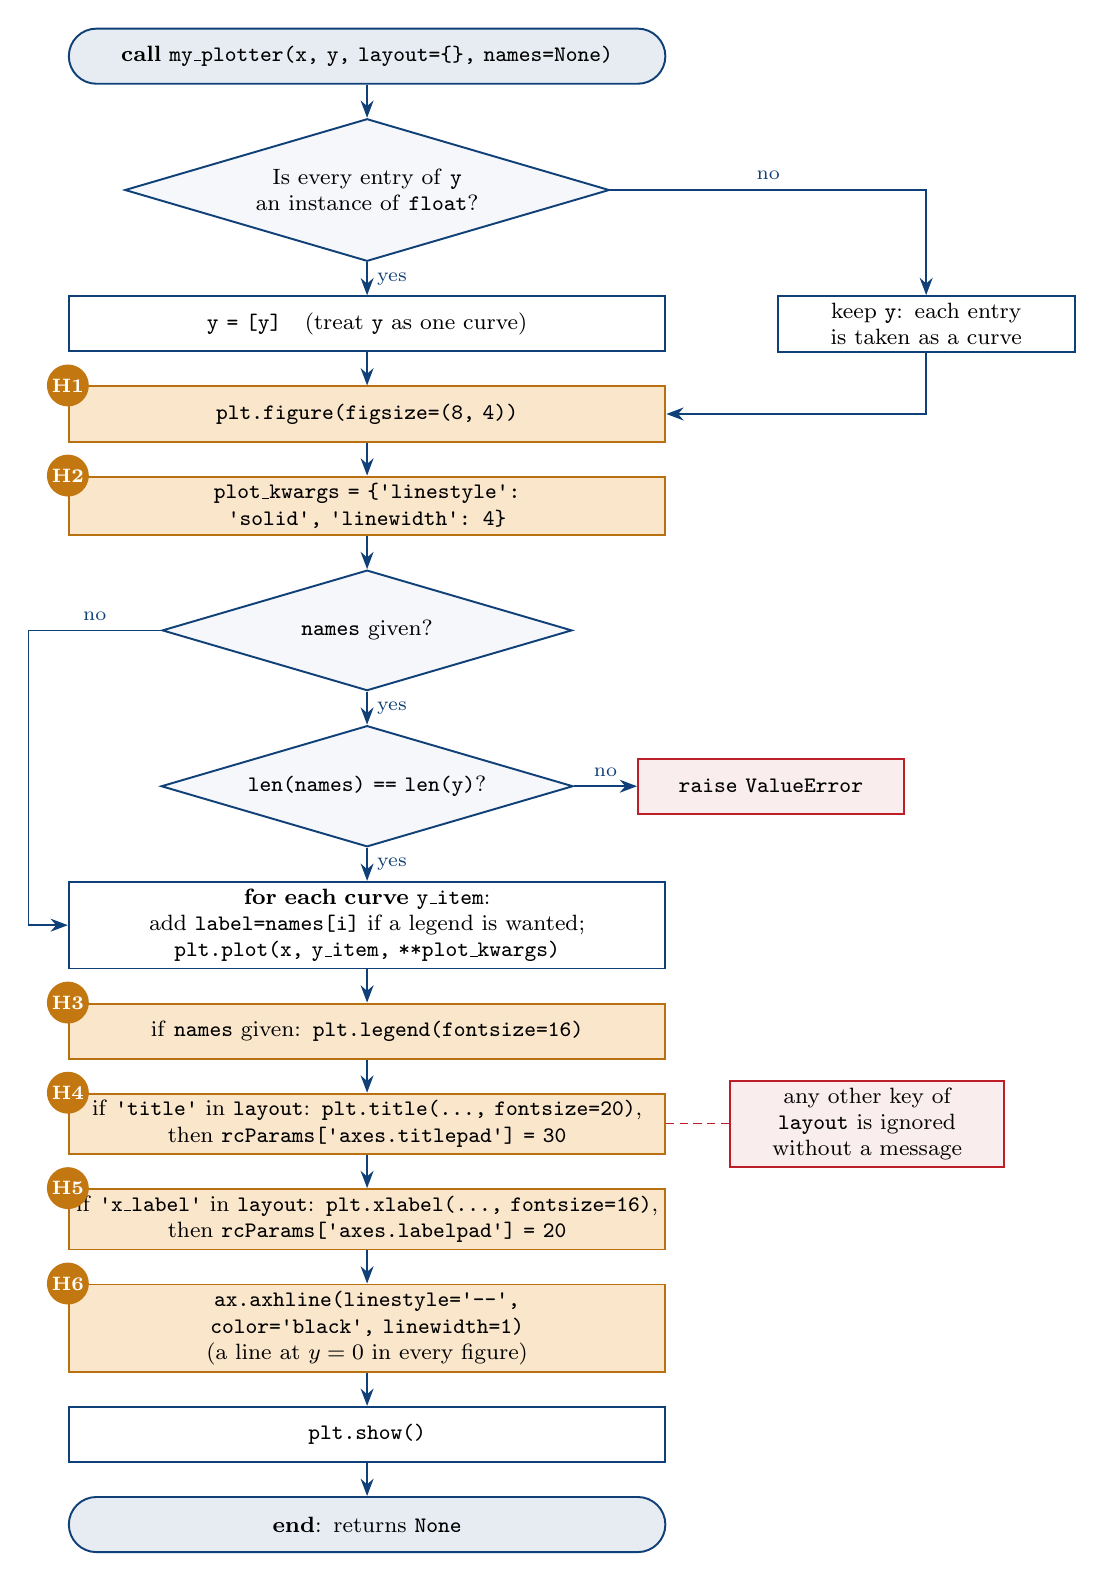
\begin{tikzpicture}[node distance=4.2mm and 6mm]
\node[fterm] (start) {\textbf{call} \texttt{my\_plotter(x, y, layout=\lb\rb, names=None)}};
\node[fdec, below=of start] (d1) {Is every entry of \texttt{y}\\ an instance of \texttt{float}?};
\node[fproc, below=of d1] (one) {\texttt{y = [y]}\quad (treat \texttt{y} as one curve)};
\node[fproc, right=14mm of one, text width=36mm] (many) {keep \texttt{y}: each entry\\ is taken as a curve};
\node[fhc, below=of one] (fig) {\texttt{plt.figure(figsize=(8, 4))}};
\node[fhc, below=of fig] (kw) {\texttt{plot\_kwargs = \lb\sq linestyle\sq: \sq solid\sq, \sq linewidth\sq: 4\rb}};
\node[fdec, below=of kw] (d2) {\texttt{names} given?};
\node[fdec, below=of d2] (d3) {\texttt{len(names) == len(y)}?};
\node[ferr, right=8mm of d3] (e1) {\texttt{raise ValueError}};
\node[fproc, below=of d3] (loop) {\textbf{for each curve} \texttt{y\_item}:\\ add \texttt{label=names[i]} if a legend is wanted;\\ \texttt{plt.plot(x, y\_item, **plot\_kwargs)}};
\node[fhc, below=of loop] (leg) {if \texttt{names} given: \texttt{plt.legend(fontsize=16)}};
\node[fhc, below=of leg] (tit) {if \texttt{\sq title\sq} in \texttt{layout}: \texttt{plt.title(..., fontsize=20)},\\ then \texttt{rcParams[\sq axes.titlepad\sq] = 30}};
\node[fhc, below=of tit] (xl) {if \texttt{\sq x\_label\sq} in \texttt{layout}: \texttt{plt.xlabel(..., fontsize=16)},\\ then \texttt{rcParams[\sq axes.labelpad\sq] = 20}};
\node[fhc, below=of xl] (hl) {\texttt{ax.axhline(linestyle=\sq-{}-\sq, color=\sq black\sq, linewidth=1)}\\ (a line at \mbox{$y=0$} in every figure)};
\node[fproc, below=of hl] (show) {\texttt{plt.show()}};
\node[fterm, below=of show] (end) {\textbf{end}: returns \texttt{None}};
\draw[farr] (start) -- (d1);
\draw[farr] (d1) -- node[flab,right]{yes} (one);
\draw[farr] (d1.east) -| node[flab,above,pos=0.25]{no} (many.north);
\draw[farr] (one) -- (fig);
\draw[farr] (many.south) |- (fig.east);
\draw[farr] (fig) -- (kw);
\draw[farr] (kw) -- (d2);
\draw[farr] (d2) -- node[flab,right]{yes} (d3);
\draw[farr] (d3) -- node[flab,above]{no} (e1);
\draw[farr] (d3) -- node[flab,right]{yes} (loop);
\draw[farr] (d2.west) -| node[flab,above,pos=0.25]{no} ([xshift=-5mm]loop.west) -- (loop.west);
\draw[farr] (loop) -- (leg);
\draw[farr] (leg) -- (tit);
\draw[farr] (tit) -- (xl);
\draw[farr] (xl) -- (hl);
\draw[farr] (hl) -- (show);
\draw[farr] (show) -- (end);
\node[tagH] at (fig.north west) {H1};
\node[tagH] at (kw.north west) {H2};
\node[tagH] at (leg.north west) {H3};
\node[tagH] at (tit.north west) {H4};
\node[tagH] at (xl.north west) {H5};
\node[tagH] at (hl.north west) {H6};
\node[ferr, right=8mm of tit, text width=33mm] (ign) {any other key of \texttt{layout} is ignored without a message};
\draw[densely dashed,draw=BUG] (ign.west) -- (tit.east);
\end{tikzpicture}
\caption{The plotter of cell 9. Orange: hard-coded layout (\tH{1}--\tH{6}).}
\label{fig:flow9}
\end{figure}

\subhead{Design.} We keep the interface of cell 9 and make the following choices.
\begin{itemize}
\item \emph{One dictionary of defaults} (\tH{1}--\tH{6}). Every layout setting is one of the $25$ keys of the dictionary \texttt{DEFAULT\_LAYOUT}, and the default of each setting of cell 9 is its value in cell 9. Hence the calls of the notebook run unchanged and, without layout options, draw the figure of cell 9: same size, curves, fonts and line at $y=0$. There are two differences: the paddings now act on the figure itself, as cell 9 intended, and \texttt{fig.tight\_layout()} shrinks the axes so that the title and the $x$-label fit inside the $8\times4$ figure. For every key $k$ the option used is
\[
\texttt{opts}[k]=
\begin{cases}
\texttt{layout}[k], & \text{if the caller gives the key } k,\\
\texttt{DEFAULT\_LAYOUT}[k], & \text{otherwise}.
\end{cases}
\]
\end{itemize}
The dictionary is in \texttt{plotter.py}; the comment \texttt{[cell 9]} marks a setting of cell 9, with the value of cell 9, and \texttt{(new)} a new option (\texttt{title} and \texttt{x\_label} are the two keys read by cell 9, and \texttt{show} decides whether \texttt{plt.show()} is called):
\par\smallskip\noindent\begin{minipage}{\linewidth}\begin{lstlisting}[style=py,title={\src{plotter.py}{27--53}}]
DEFAULT_LAYOUT: Dict[str, Any] = {
    "figsize": (8, 4),        # inches (width, height)              [cell 9]
    "title": None,            # title of the axes
    "x_label": None,          # x-axis label
    "y_label": None,          # y-axis label                        (new)
    "title_fontsize": 20,     #                                     [cell 9]
    "label_fontsize": 16,     # x- and y-label                      [cell 9]
    "legend_fontsize": 16,    #                                     [cell 9]
    "tick_fontsize": None,    # None: Matplotlib default            [cell 9]
    "title_pad": 30,          # points between title and axes       [cell 9]
    "label_pad": 20,          # points between label and axis       [cell 9]
    "linewidth": 4,           #                                     [cell 9]
    "colors": None,           # colour or list, cycled over curves  (new)
    "linestyles": "solid",    # style or list like ["-", "--"]      [cell 9]
    "markers": None,          # marker or list like [None, "o"]     (new)
    "alpha": 1.0,             # opacity of the curves               (new)
    "legend_loc": "best",     # position of the legend              (new)
    "grid": False,            # True: light dashed grid             (new)
    "hline": 0.0,             # y of the dashed black line, or None [cell 9]
    "vlines": None,           # x values of dotted vertical lines   (new)
    "xlim": None,             # (xmin, xmax)                        (new)
    "ylim": None,             # (ymin, ymax)                        (new)
    "logx": False,            # logarithmic x-axis                  (new)
    "logy": False,            # logarithmic y-axis                  (new)
    "save_path": None,        # e.g. "figures/plot.pdf"             (new)
    "show": None,             # None: show only a figure created here
}
\end{lstlisting}\end{minipage}\par\smallskip
The merge rule above, with the \texttt{KeyError} for unknown keys, is the start of \texttt{my\_plotter}:
\par\smallskip\noindent\begin{minipage}{\linewidth}\begin{lstlisting}[style=py,title={\src{plotter.py}{77--82}}]
    opts = dict(DEFAULT_LAYOUT)
    for key, value in (layout or {}).items():
        if key not in DEFAULT_LAYOUT:
            raise KeyError(f"unknown layout key {key!r}; "
                           f"allowed keys: {sorted(DEFAULT_LAYOUT)}")
        opts[key] = value
\end{lstlisting}\end{minipage}\par\smallskip
Figure~\ref{fig:flownew} follows the new function; the green tags show where each hard-coded value of Figure~\ref{fig:flow9} went.

\begin{figure}[p]
\centering
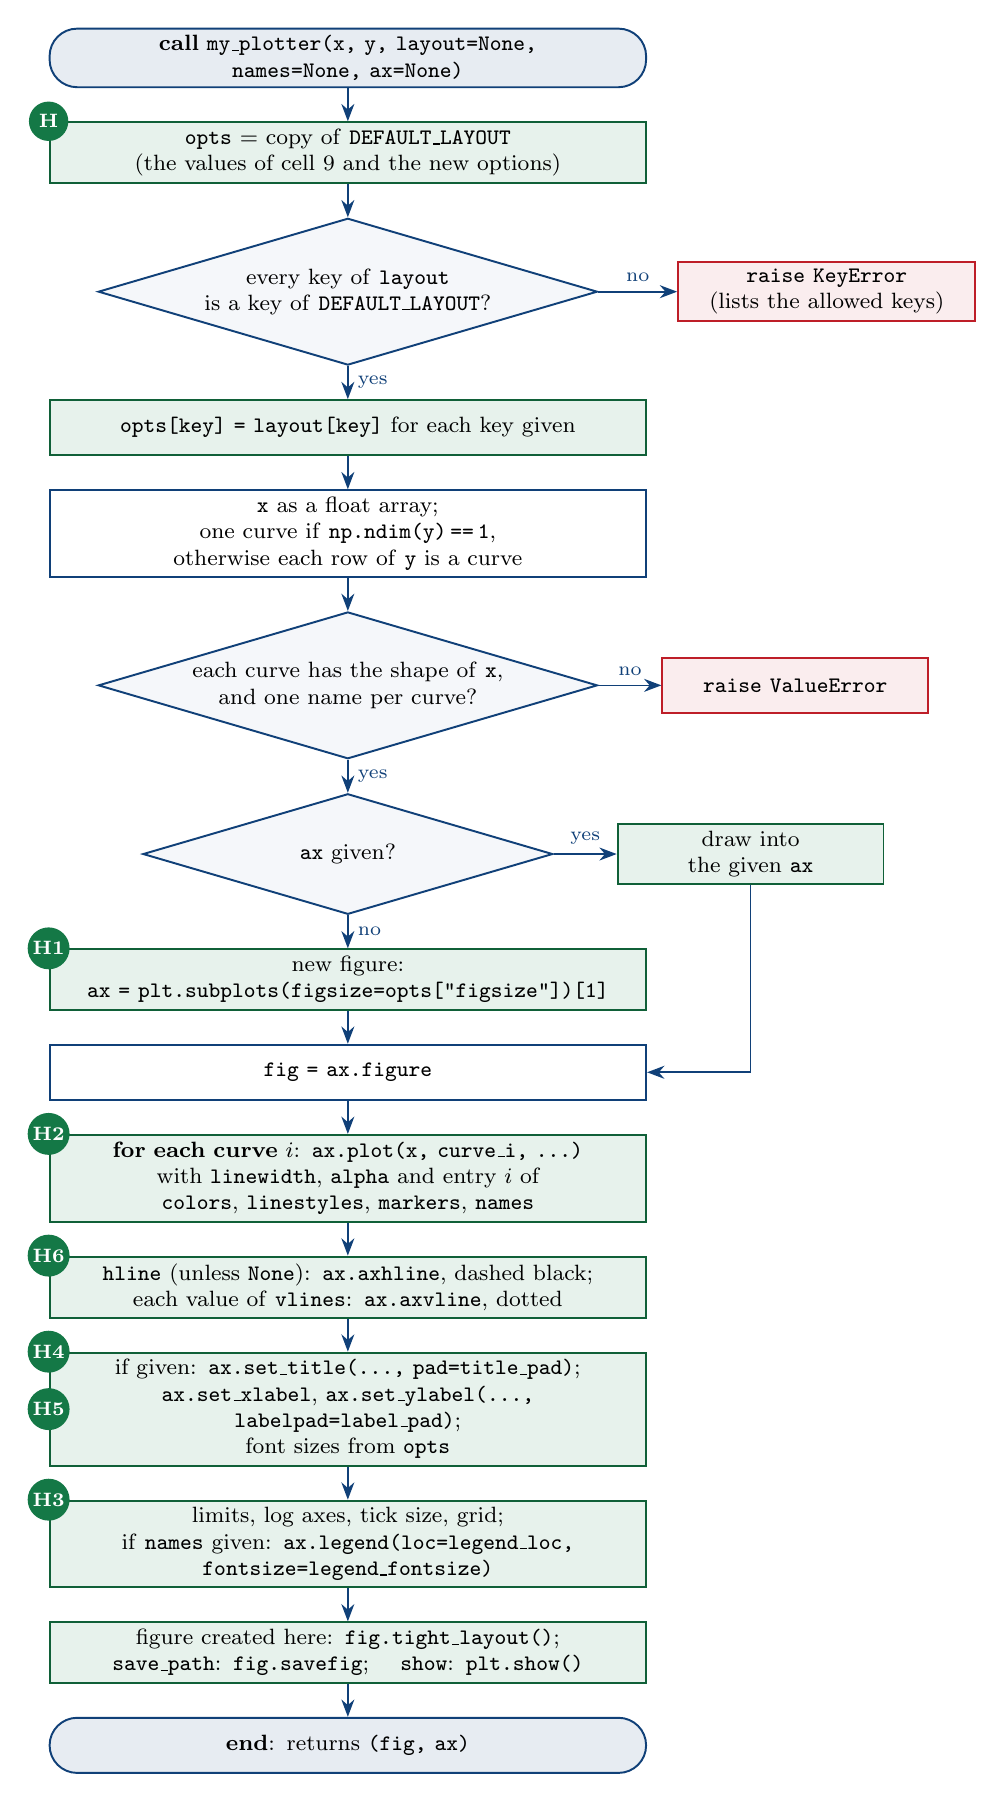
\begin{tikzpicture}[node distance=4.2mm and 6mm]
\node[fterm] (start) {\textbf{call} \texttt{my\_plotter(x, y, layout=None, names=None, ax=None)}};
\node[fnew, below=of start] (opts) {\texttt{opts} = copy of \texttt{DEFAULT\_LAYOUT}\\ (the values of cell 9 and the new options)};
\node[fdec, below=of opts] (dk) {every key of \texttt{layout}\\ is a key of \texttt{DEFAULT\_LAYOUT}?};
\node[ferr, right=10mm of dk, text width=36mm] (ek) {\texttt{raise KeyError}\\ (lists the allowed keys)};
\node[fnew, below=of dk] (merge) {\texttt{opts[key] = layout[key]} for each key given};
\node[fproc, below=of merge] (data) {\texttt{x} as a float array;\\ one curve if \texttt{np.ndim(y)\,==\,1},\\ otherwise each row of \texttt{y} is a curve};
\node[fdec, below=of data] (dd) {each curve has the shape of \texttt{x},\\ and one name per curve?};
\node[ferr, right=8mm of dd] (ev) {\texttt{raise ValueError}};
\node[fdec, below=of dd] (dax) {\texttt{ax} given?};
\node[fnew, right=8mm of dax, text width=32mm] (given) {draw into\\ the given \texttt{ax}};
\node[fnew, below=of dax] (newfig) {new figure:\\ \texttt{ax = plt.subplots(figsize=opts["figsize"])[1]}};
\node[fproc, below=of newfig] (join) {\texttt{fig = ax.figure}};
\node[fnew, below=of join] (plot) {\textbf{for each curve} $i$: \texttt{ax.plot(x, curve\_i, ...)}\\ with \texttt{linewidth}, \texttt{alpha} and entry $i$ of\\ \texttt{colors}, \texttt{linestyles}, \texttt{markers}, \texttt{names}};
\node[fnew, below=of plot] (lines) {\texttt{hline} (unless \texttt{None}): \texttt{ax.axhline}, dashed black;\\ each value of \texttt{vlines}: \texttt{ax.axvline}, dotted};
\node[fnew, below=of lines] (text) {if given: \texttt{ax.set\_title(..., pad=title\_pad)};\\ \texttt{ax.set\_xlabel}, \texttt{ax.set\_ylabel(..., labelpad=label\_pad)};\\ font sizes from \texttt{opts}};
\node[fnew, below=of text] (axes) {limits, log axes, tick size, grid;\\ if \texttt{names} given: \texttt{ax.legend(loc=legend\_loc,}\\ \texttt{fontsize=legend\_fontsize)}};
\node[fnew, below=of axes] (out) {figure created here: \texttt{fig.tight\_layout()};\\ \texttt{save\_path}: \texttt{fig.savefig}; \quad \texttt{show}: \texttt{plt.show()}};
\node[fterm, below=of out] (end) {\textbf{end}: returns \texttt{(fig, ax)}};
\draw[farr] (start) -- (opts);
\draw[farr] (opts) -- (dk);
\draw[farr] (dk) -- node[flab,above]{no} (ek);
\draw[farr] (dk) -- node[flab,right]{yes} (merge);
\draw[farr] (merge) -- (data);
\draw[farr] (data) -- (dd);
\draw[farr] (dd) -- node[flab,above]{no} (ev);
\draw[farr] (dd) -- node[flab,right]{yes} (dax);
\draw[farr] (dax) -- node[flab,above]{yes} (given);
\draw[farr] (dax) -- node[flab,right]{no} (newfig);
\draw[farr] (given.south) |- (join.east);
\draw[farr] (newfig) -- (join);
\draw[farr] (join) -- (plot);
\draw[farr] (plot) -- (lines);
\draw[farr] (lines) -- (text);
\draw[farr] (text) -- (axes);
\draw[farr] (axes) -- (out);
\draw[farr] (out) -- (end);
\node[tagF] at (opts.north west) {H};
\node[tagF] at (newfig.north west) {H1};
\node[tagF] at (plot.north west) {H2};
\node[tagF] at (lines.north west) {H6};
\node[tagF] at (text.north west) {H4};
\node[tagF] at (text.west) {H5};
\node[tagF] at (axes.north west) {H3};
\end{tikzpicture}
\caption{The new \texttt{my\_plotter} of \texttt{plotter.py}. Green boxes use the options \texttt{opts}; green tags: where the hard-coded values \tH{1}--\tH{6} of Figure~\ref{fig:flow9} went (\tF{H}: all of them, as defaults).}
\label{fig:flownew}
\end{figure}

\subhead{The same call with the new plotter.} After \texttt{from plotter import my\_plotter}, the call of cell 11 runs unchanged; we only keep the returned pair:
\par\smallskip\noindent\begin{minipage}{\linewidth}\begin{lstlisting}[style=py,title={\src{hw21\_examples.py}{30--35} (block 2)}]
from plotter import my_plotter          # the new plotter replaces cell 9

fig, ax = my_plotter(x_stock_price, [y_forward_payoff, y_forward_payoff__short],
                     layout=layout,
                     names=['Long Forward Payoff at time $T$',
                            'Short Forward Payoff at time $T$'])
\end{lstlisting}\end{minipage}\par\smallskip
\emph{What it shows} is Figure~\ref{fig:newout}. Compared with Figure~\ref{fig:cell9out}, the figure size, the curves, the colours, the font sizes and the line at $y=0$ are the same, because these are the defaults. The title and the $x$-label are further from the axes: the new plotter applies the paddings $30$ and $20$ of cell 9 to this figure, while cell 9, in its first call, still draws with the default paddings (from its second call on, cell 9 also uses $30$ and $20$).
\begin{figure}[!ht]
\centering
\resizebox{0.62\textwidth}{!}{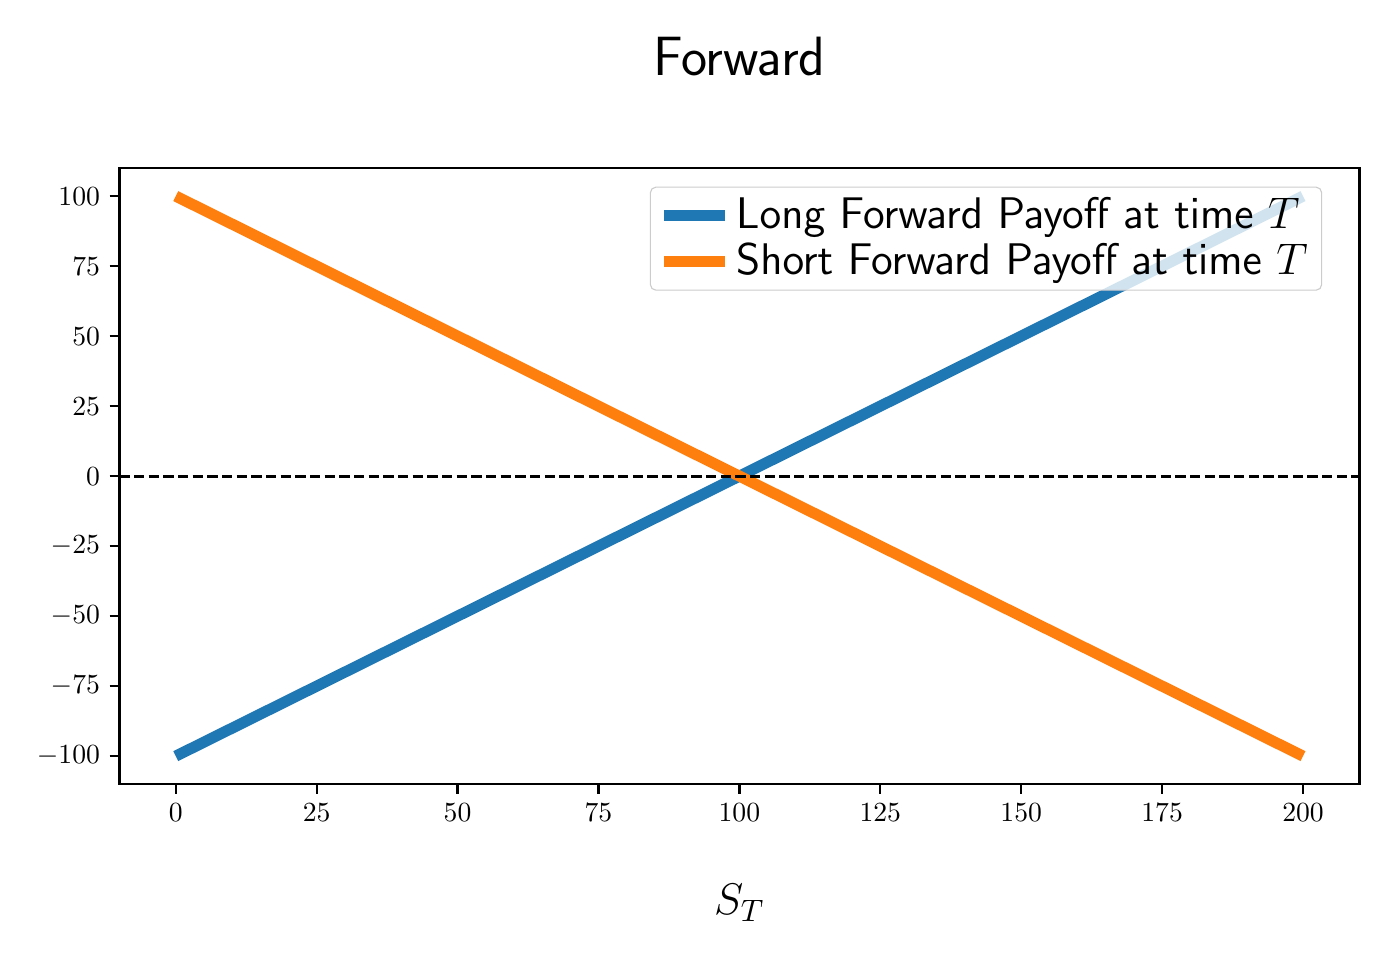
\begin{tikzpicture}
\begin{axis}[mpl, width=6.2in, height=3.08in, xmin=-10, xmax=210, ymin=-110, ymax=110,
  xtick={0,25,...,200}, ytick={-100,-75,...,100},
  title={\fontsize{20}{24}\selectfont\sffamily Forward}, title style={yshift=24pt},
  xlabel={\fontsize{16}{19}\selectfont $S_{T}$}, xlabel style={yshift=-16pt},
  legend pos=north east, legend style={font=\fontsize{16}{19}\selectfont\sffamily}]
\addplot[tabblue, line width=4pt] coordinates {(0,-100) (199.999,99.999)};
\addlegendentry{Long Forward Payoff at time $T$}
\addplot[taborange, line width=4pt] coordinates {(0,100) (199.999,-99.999)};
\addlegendentry{Short Forward Payoff at time $T$}
\draw[black, line width=1pt, mpldash] (axis cs:-10,0) -- (axis cs:210,0);
\end{axis}
\end{tikzpicture}}
\caption{Output of block 2: the call of cell 11 with the new plotter and no layout options except the title and the $x$-label of cell 11.}
\label{fig:newout}
\end{figure}

\subhead{How to use the new features.} Each feature is a key of \texttt{DEFAULT\_LAYOUT}. The caller gives only the keys he wants to change, and the function passes each value to one Matplotlib command (Table~\ref{tab:features}). For \texttt{colors}, \texttt{linestyles} and \texttt{markers} a list is cycled over the curves: curve $i$ gets the entry $i \bmod (\text{length of the list})$, so \texttt{["-", "--"]} alternates solid and dashed curves; a single string, such as \texttt{"red"}, applies to all curves.

\begin{table}[!ht]
\centering\small
\caption{The new features of \texttt{my\_plotter}: the key, an example value and the Matplotlib command that uses it.}
\label{tab:features}
\begin{tabular}{@{}llll@{}}
\toprule
group & key & example value & passed to\\
\midrule
labels & \texttt{y\_label} & \texttt{"value at \char36T\char36"} & \texttt{ax.set\_ylabel}\\
 & \texttt{tick\_fontsize} & \texttt{10} & \texttt{ax.tick\_params(labelsize=...)}\\
\addlinespace
curves & \texttt{colors} & \texttt{["tab:blue", "tab:red"]} & \texttt{color=} of \texttt{ax.plot}\\
 & \texttt{linestyles} & \texttt{["-", "--"]} & \texttt{linestyle=} of \texttt{ax.plot}\\
 & \texttt{markers} & \texttt{[None, "o"]} & \texttt{marker=} of \texttt{ax.plot}\\
 & \texttt{alpha} & \texttt{0.6} & \texttt{alpha=} of \texttt{ax.plot}\\
\addlinespace
axes & \texttt{legend\_loc} & \texttt{"upper center"} & \texttt{ax.legend(loc=...)}\\
 & \texttt{grid} & \texttt{True} & \texttt{ax.grid}\\
 & \texttt{hline} & \texttt{None} (no line) or \texttt{5.0} & \texttt{ax.axhline}\\
 & \texttt{vlines} & \texttt{[92, 105]} & \texttt{ax.axvline}, once per value\\
 & \texttt{xlim}, \texttt{ylim} & \texttt{(-15, 100)} & \texttt{ax.set\_xlim}, \texttt{ax.set\_ylim}\\
 & \texttt{logx}, \texttt{logy} & \texttt{True} & \texttt{ax.set\_xscale("log")}, \texttt{ax.set\_yscale("log")}\\
\addlinespace
output & \texttt{save\_path} & \texttt{"payoffs.pdf"} & \texttt{fig.savefig}\\
 & \texttt{show} & \texttt{False} & \texttt{True}: always \texttt{plt.show()};\\
 & & & default \texttt{None}: only for a figure created here\\
 & argument \texttt{ax} & \texttt{axes[0]} & draws into that subplot\\
 & return value & \texttt{fig, ax = my\_plotter(...)} & the figure stays editable\\
\bottomrule
\end{tabular}
\end{table}

\noindent For example, two plots side by side in one figure, saved to a file (a figure made by the caller keeps its layout, so the caller applies \texttt{fig.tight\_layout()}); it shows Figure~\ref{fig:subout}:
\par\smallskip\noindent\begin{minipage}{\linewidth}\begin{lstlisting}[style=py,title={\src{hw21\_examples.py}{38--49} (block 3)}]
x = np.arange(0, 200, 0.001)
call_payoff = np.maximum(x - 100, 0.0)
put_payoff = np.maximum(100 - x, 0.0)

fig, axes = plt.subplots(1, 2, figsize=(12, 4))
my_plotter(x, [call_payoff, put_payoff], ax=axes[0], names=["call", "put"],
           layout={"title": "Payoffs", "colors": ["tab:blue", "tab:red"]})
my_plotter(x, put_payoff - 8, ax=axes[1], layout={"title": "Put net profit",
           "hline": None, "vlines": [92], "grid": True})
fig.tight_layout()
fig.savefig("figures/hw21_subplots.pdf")
plt.show()
\end{lstlisting}\end{minipage}\par\smallskip
\begin{figure}[!ht]
\centering
\resizebox{0.9\textwidth}{!}{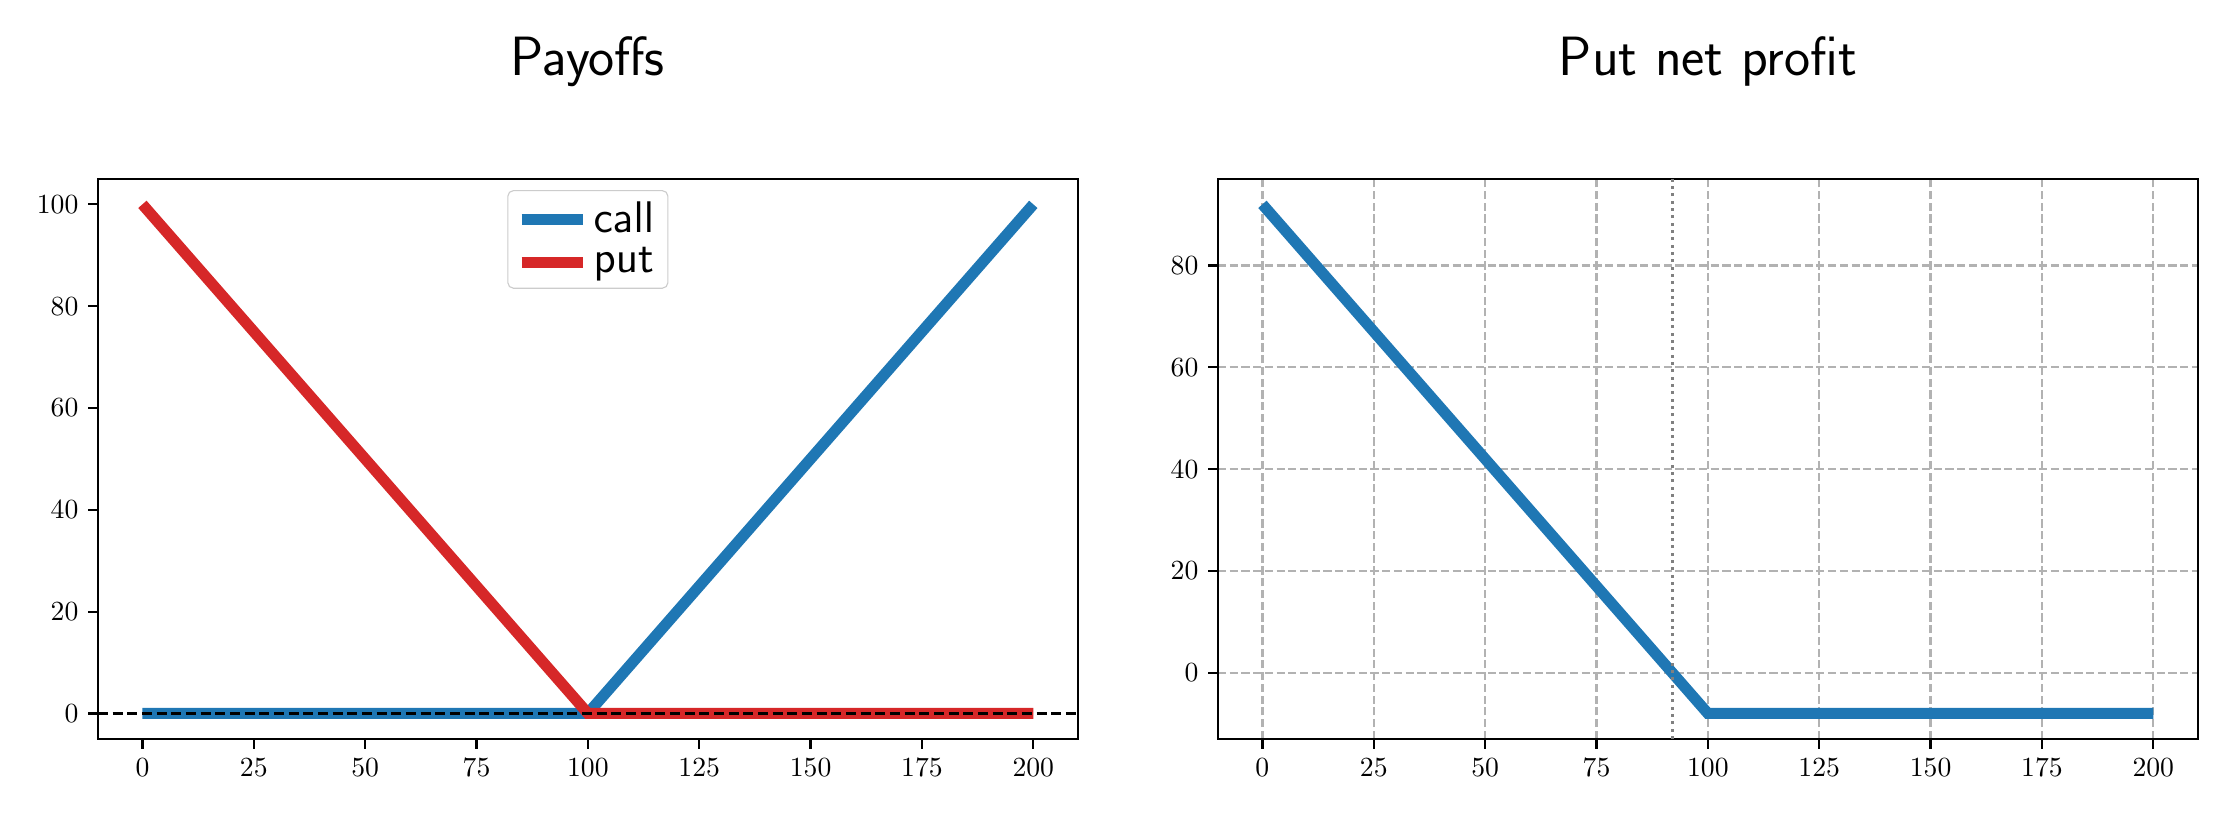
\begin{tikzpicture}
\begin{axis}[mpl, width=4.9in, height=2.8in, xmin=-10, xmax=210, ymin=-5, ymax=105,
  xtick={0,25,...,200}, ytick={0,20,...,100},
  title={\fontsize{20}{24}\selectfont\sffamily Payoffs}, title style={yshift=24pt},
  legend style={at={(0.5,0.98)}, anchor=north, font=\fontsize{16}{19}\selectfont\sffamily}]
\addplot[tabblue, line width=4pt] coordinates {(0,0) (100,0) (199.999,99.999)};
\addlegendentry{call}
\addplot[tabred, line width=4pt] coordinates {(0,100) (100,0) (199.999,0)};
\addlegendentry{put}
\draw[black, line width=1pt, mpldash] (axis cs:-10,0) -- (axis cs:210,0);
\end{axis}
\begin{axis}[mpl, mplgrid, xshift=5.6in, width=4.9in, height=2.8in, xmin=-10, xmax=210, ymin=-13, ymax=97,
  xtick={0,25,...,200}, ytick={0,20,...,80},
  title={\fontsize{20}{24}\selectfont\sffamily Put net profit}, title style={yshift=24pt}]
\addplot[tabblue, line width=4pt] coordinates {(0,92) (100,-8) (199.999,-8)};
\draw[black!50, line width=1pt, mpldot] (axis cs:92,-13) -- (axis cs:92,97);
\end{axis}
\end{tikzpicture}}
\caption{Output of block 3: two calls of the new plotter drawing into the two axes of one figure.}
\label{fig:subout}
\end{figure}

\subhead{Example.} Figure~\ref{fig:payoffs} is drawn by one call of the new plotter with the data of cells 10, 19 and 25 ($K=100$, call premium $5$, put premium $8$; cell 25 subtracts \texttt{call\_price} from the put payoff by mistake; here the put premium is used). Its options are grouped as in Table~\ref{tab:features}; the code continues block 3 (it uses \texttt{x}, \texttt{call\_payoff}, \texttt{put\_payoff}) and shows Figure~\ref{fig:payoffs}:
\par\smallskip\noindent\begin{minipage}{\linewidth}\begin{lstlisting}[style=py,title={\src{hw21\_examples.py}{52--71} (block 4)}]
call_price, put_price = 5.0, 8.0        # premiums of cells 19 and 25
example_layout = {
    # text: title, axis labels, sizes and paddings
    "title": "Long call and long put, K = 100", "title_fontsize": 13,
    "x_label": "$S_T$", "y_label": "value at $T$", "label_fontsize": 12,
    "title_pad": 12, "label_pad": 8, "tick_fontsize": 10,
    # curves: one entry per curve (a list is cycled over the curves)
    "colors": ["tab:blue", "tab:blue", "tab:red", "tab:red"],
    "linestyles": ["-", "--", "-", "--"], "linewidth": 2.2,
    # axes: reference lines, limits, grid and legend
    "hline": None, "vlines": [92, 105], "ylim": (-15, 100), "grid": True,
    "legend_loc": "upper center", "legend_fontsize": 9,
    # output: figure size and file
    "figsize": (7.5, 3.8), "save_path": "figures/hw21_payoffs.pdf",
}
fig, ax = my_plotter(x, [call_payoff, call_payoff - call_price,
                         put_payoff, put_payoff - put_price],
                     layout=example_layout,
                     names=["call payoff", "call net profit (c = 5)",
                            "put payoff", "put net profit (p = 8)"])
\end{lstlisting}\end{minipage}\par\smallskip

\begin{figure}[!ht]
\centering
\resizebox{0.7\textwidth}{!}{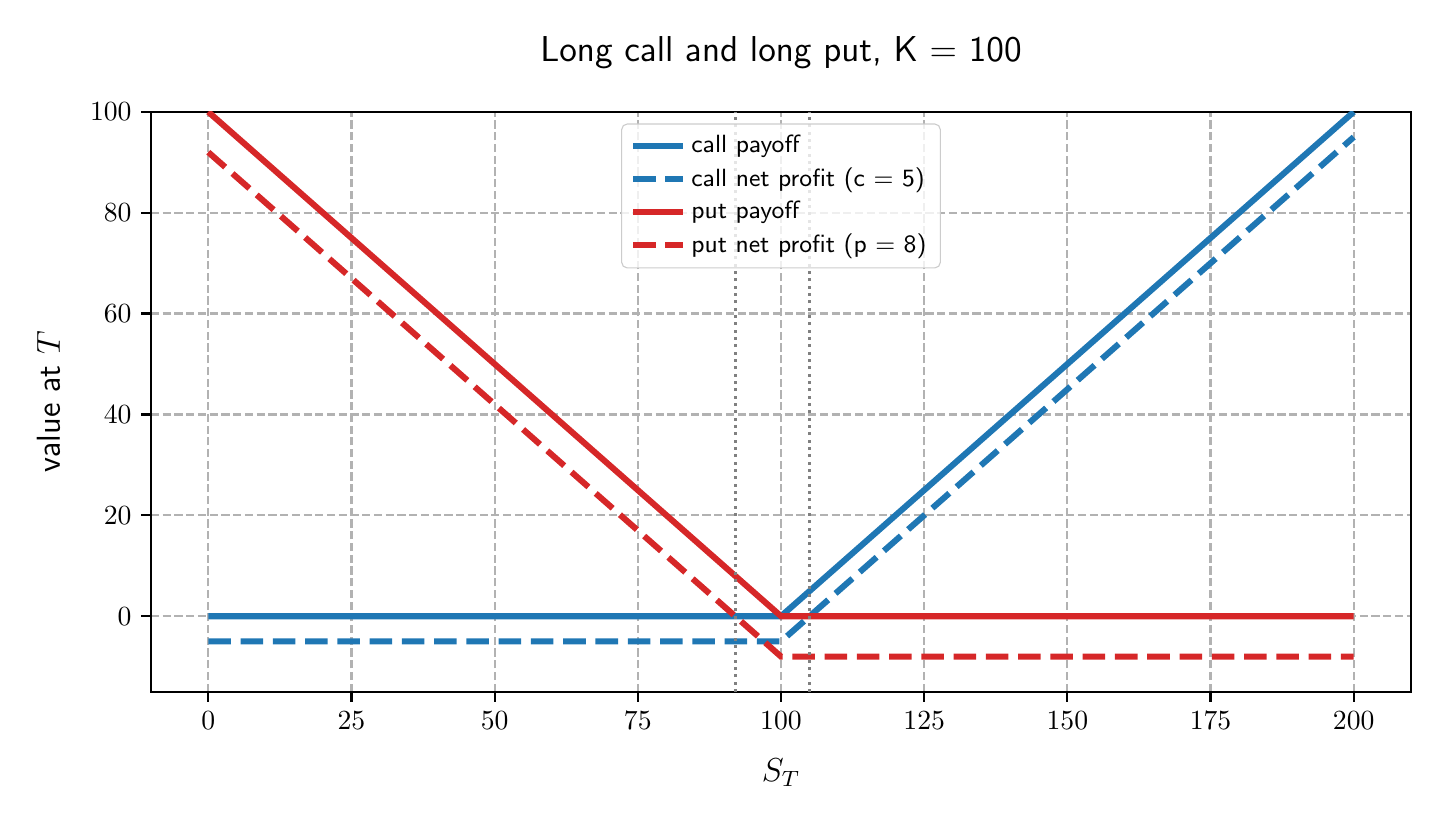
\begin{tikzpicture}
\begin{axis}[mpl, mplgrid, width=6.3in, height=2.9in, xmin=-10, xmax=210, ymin=-15, ymax=100,
  xtick={0,25,...,200}, ytick={0,20,...,100},
  title={\fontsize{13}{16}\selectfont\sffamily Long call and long put, K = 100}, title style={yshift=6pt},
  xlabel={\fontsize{12}{14}\selectfont $S_T$}, ylabel={\fontsize{12}{14}\selectfont\sffamily value at $T$},
  xlabel style={yshift=-4pt}, ylabel style={yshift=4pt},
  legend style={at={(0.5,0.98)}, anchor=north, font=\fontsize{9}{11}\selectfont\sffamily},
  legend image code/.code={\draw[#1] (0pt,0pt) -- (18pt,0pt);}]
\addplot[tabblue, line width=2.2pt] coordinates {(0,0) (100,0) (199.999,99.999)};
\addlegendentry{call payoff}
\addplot[tabblue, line width=2.2pt, dash pattern=on 8.14pt off 3.52pt] coordinates {(0,-5) (100,-5) (199.999,94.999)};
\addlegendentry{call net profit (c = 5)}
\addplot[tabred, line width=2.2pt] coordinates {(0,100) (100,0) (199.999,0)};
\addlegendentry{put payoff}
\addplot[tabred, line width=2.2pt, dash pattern=on 8.14pt off 3.52pt] coordinates {(0,92) (100,-8) (199.999,-8)};
\addlegendentry{put net profit (p = 8)}
\draw[black!50, line width=1pt, mpldot] (axis cs:92,-15) -- (axis cs:92,100);
\draw[black!50, line width=1pt, mpldot] (axis cs:105,-15) -- (axis cs:105,100);
\end{axis}
\end{tikzpicture}}
\caption{Output of block 4. Payoffs (solid) and net profits (dashed; payoff minus premium, cells 19--20 and 25--26) of a long call (blue, premium $5$) and a long put (red, premium $8$) with $K=100$, drawn with the new plotter. The dotted lines (option \texttt{vlines}) are at the break-even points $S_T=100+5=105$ and $S_T=100-8=92$.}
\label{fig:payoffs}
\end{figure}

\subhead{Check.} Running the four blocks of \texttt{hw21\_examples.py} as printed here and testing the new plotter gives:
\begin{itemize}
\item block 1 shows the array above and Figure~\ref{fig:cell9out}, and cell 9 changes the global paddings to $30/20$ only after its first figure; block 2 draws the same size, curves, colours and fonts with paddings $30/20$; block 3 saves a figure with two panels;
\item \texttt{DEFAULT\_LAYOUT} has $25$ keys; Figure~\ref{fig:payoffs} has $4$ curves and $2$ vertical lines, and the net profits vanish at $S_T=105$ (call) and $S_T=92$ (put);
\item without layout options: figure size $(8,4)$, solid lines of width $4$, font sizes $20/16/16$, paddings $30/20$ on the figure itself, a dashed line at $y=0$ and no grid, as in cell 9;
\item the unknown key \texttt{"colour"} raises \texttt{KeyError}; two curves with one name, and \texttt{x}, \texttt{y} of lengths $3$ and $2$, raise \texttt{ValueError};
\item \texttt{np.arange(5)} as both \texttt{x} and \texttt{y} is drawn as one curve, and \texttt{rcParams} is the same before and after a call with a title and an $x$-label;
\item two calls with \texttt{ax=axes[0]} and \texttt{ax=axes[1]} draw into one figure.
\end{itemize}

\ansbox{Hence the plotter of cell 9 is replaced by
\[
\texttt{my\_plotter(x, y, layout=None, names=None, ax=None)},
\]
which returns \texttt{(fig, ax)}. All $25$ layout settings of \texttt{DEFAULT\_LAYOUT} can be customized through \texttt{layout}; their defaults are the values of cell 9, so the notebook calls run unchanged and draw the same curves, fonts and sizes (with \texttt{tight\_layout}). Unknown keys raise \texttt{KeyError}, data of the wrong shape raise \texttt{ValueError}, integer input works and no global \texttt{rcParams} are changed. New features: $y$-label, tick size, colours, line styles, markers, opacity, legend position, grid, reference lines, limits, log axes, saving, subplots.}

% ============================================================================ HW 2/2
\bigskip
\begin{thmbox}{Black--Scholes--Merton price of a European call; Lesson 3, cells 37, 48}
The price at time $0$ of a European call with strike $K$ and maturity $T$ on a non-dividend-paying stock is
\begin{equation}\label{eq:call}
c=S_0\,N(d_1)-K e^{-rT}N(d_2),
\end{equation}
where $N$ is the distribution function of the standard normal distribution and
\begin{equation}\label{eq:d1d2}
d_1=\frac{\ln(S_0/K)+(r+\sigma^2/2)\,T}{\sigma\sqrt{T}},\qquad d_2=d_1-\sigma\sqrt{T}.
\end{equation}
\end{thmbox}

\begin{thmbox}{Greeks of the European call; Lesson 3, cells 46--49}
With $N'$ the density of the standard normal distribution and $d_1,d_2$ as in \eqref{eq:d1d2}, the Greeks of the call at time $0$ (cell 49 with $t=0$) are
\begin{equation}\label{eq:callgreeks}
\begin{aligned}
\Delta&=N(d_1), &\Gamma&=\frac{N'(d_1)}{S_0\,\sigma\sqrt{T}}, &\mathcal V&=S_0\,N'(d_1)\sqrt{T},\\
\Theta&=-\frac{S_0\,N'(d_1)\,\sigma}{2\sqrt{T}}-rKe^{-rT}N(d_2), &\rho&=KTe^{-rT}N(d_2).
\end{aligned}
\end{equation}
\end{thmbox}

\needspace{8\baselineskip}
\begin{exercise}{HW 2/2}
Upgrade the BSM call option pricer to be able to return the greeks as well, not just the price.
\end{exercise}
\solution
\subhead{What is asked.} The pricer of cell 43 returns only the price, Theorem~1, \eqref{eq:call}. It must also be able to return the Greeks of Theorem~2, \eqref{eq:callgreeks}.

\subhead{A problem in cell 43.} The return line of cell 43 uses \texttt{K\_vec}, the global variable of cell 44, and not the argument \texttt{K}. Cell 44 still works, because there \texttt{K=K\_vec}, but one strike gives $2000$ numbers:
\par\smallskip\noindent\begin{minipage}{\linewidth}\begin{lstlisting}[style=py,title={professor's cell 43, run after cell 44}]
# test: one strike K = 20.0 should give one price
c = black_scholes_eur_call(r=0.05, T=1.0, S0=20.0, sigma=0.3, K=20.0)
print(c.shape)
print(c[:3])
\end{lstlisting}
\begin{lstlisting}[style=out,title={output}]
(2000,)
[7.66564276 7.66082337 7.65600397]
\end{lstlisting}\end{minipage}\par\smallskip

\subhead{New version.} The code of cell 43 with two changes (the lines of cell 43 that are replaced are kept as \texttt{\#Delete.} comments):
\begin{itemize}
\item \texttt{change \# 1}: the return line uses the argument \texttt{K}, and the price is stored in \texttt{price};
\item \texttt{change \# 2}: a new argument \texttt{return\_greeks}. With the default \texttt{False} the function returns the price, as before, so cell 44 runs unchanged; with \texttt{True} it returns a dictionary with the price and the five Greeks of Theorem~2, \eqref{eq:callgreeks}.
\end{itemize}
\par\smallskip\noindent\begin{minipage}{\linewidth}\begin{lstlisting}[style=prof,title={new version of cell 43}]
import numpy as np
import matplotlib.pyplot as plt
from scipy.stats import norm
from typing import Dict, List, Union

"""The pricing function of European call option"""
# change # 2
#Delete.    def black_scholes_eur_call(r: float, T: float, S0: float, sigma: float,
#Delete.                               K: Union[float, List[float], np.ndarray]) -> np.ndarray:
# replace by
def black_scholes_eur_call(r: float, T: float, S0: float, sigma: float,
                           K: Union[float, List[float], np.ndarray],
                           return_greeks: bool = False):
# end change # 2
    """
    Black-Scholes pricer of European call option on non-dividend-paying stock

    param r: risk-free interest rate (which is constant)
    param T: time to maturity (in years)
    param S0: initial spot price of the underlying stock
    param sigma: volatility of the underlying stock
    param K: strike price (or prices)
    param return_greeks: if True, return a dict with the price and the greeks
    """
    # check conditions
    assert sigma > 0

    K = np.array([K]) if isinstance(K, float) else np.array(K)

    d1_vec = ( np.log( S0 / K ) + ( r + 0.5 * sigma**2 ) * T ) / ( sigma * T**0.5 )
    d2_vec = d1_vec - sigma * T**0.5

    N_d1_vec = norm.cdf(d1_vec)
    N_d2_vec = norm.cdf(d2_vec)

    # change # 1
    #Delete.    return N_d1_vec * S0 - K_vec * np.exp((-1.0)*r*T) * N_d2_vec
    # replace by
    price = N_d1_vec * S0 - K * np.exp((-1.0)*r*T) * N_d2_vec
    # end change # 1

    # change # 2
    if not return_greeks:
        return price
    n_d1_vec = norm.pdf(d1_vec)                  # N'(d1)
    return {
        "price": price,
        "delta": N_d1_vec,
        "gamma": n_d1_vec / (S0 * sigma * T**0.5),
        "vega":  S0 * n_d1_vec * T**0.5,
        "theta": -S0 * n_d1_vec * sigma / (2 * T**0.5) - r * K * np.exp(-r*T) * N_d2_vec,
        "rho":   K * T * np.exp(-r*T) * N_d2_vec,
    }
    # end change # 2
\end{lstlisting}\end{minipage}\par\smallskip

\subhead{Test.} One strike gives one price, and the running example $S_0=K=100$, $r=0.05$, $\sigma=0.2$, $T=1$ gives the price and the Greeks:
\par\smallskip\noindent\begin{minipage}{\linewidth}\begin{lstlisting}[style=py,title={test of the new version}]
# test 1: one strike gives one price
print(black_scholes_eur_call(r=0.05, T=1.0, S0=20.0, sigma=0.3, K=20.0))

# test 2: price and greeks, S0 = K = 100, r = 0.05, sigma = 0.2, T = 1
g = black_scholes_eur_call(r=0.05, T=1.0, S0=100.0, sigma=0.2, K=100.0,
                           return_greeks=True)
for name, value in g.items():
    print(name, round(float(value[0]), 6))
\end{lstlisting}
\begin{lstlisting}[style=out,title={output}]
[2.84625096]
price 10.450584
delta 0.636831
gamma 0.018762
vega 37.524035
theta -6.414028
rho 53.232482
\end{lstlisting}\end{minipage}\par\smallskip
By hand, \eqref{eq:d1d2} gives
\begin{align*}
d_1 &= \frac{\ln 1+(0.05+0.02)\cdot 1}{0.2}\\
&= 0.35,\\
d_2 &= 0.35-0.2\\
&= 0.15,
\end{align*}
and \eqref{eq:call} gives
\begin{align*}
c &= 100\,N(0.35)-100\,e^{-0.05}N(0.15)\\
&\approx 63.6831-53.2325\\
&= 10.4506, && \checkmark
\end{align*}
the price printed above. Cell 44, run unchanged with the new version, draws Figure~\ref{fig:call}.

\begin{figure}[!ht]
\centering
\resizebox{0.7\textwidth}{!}{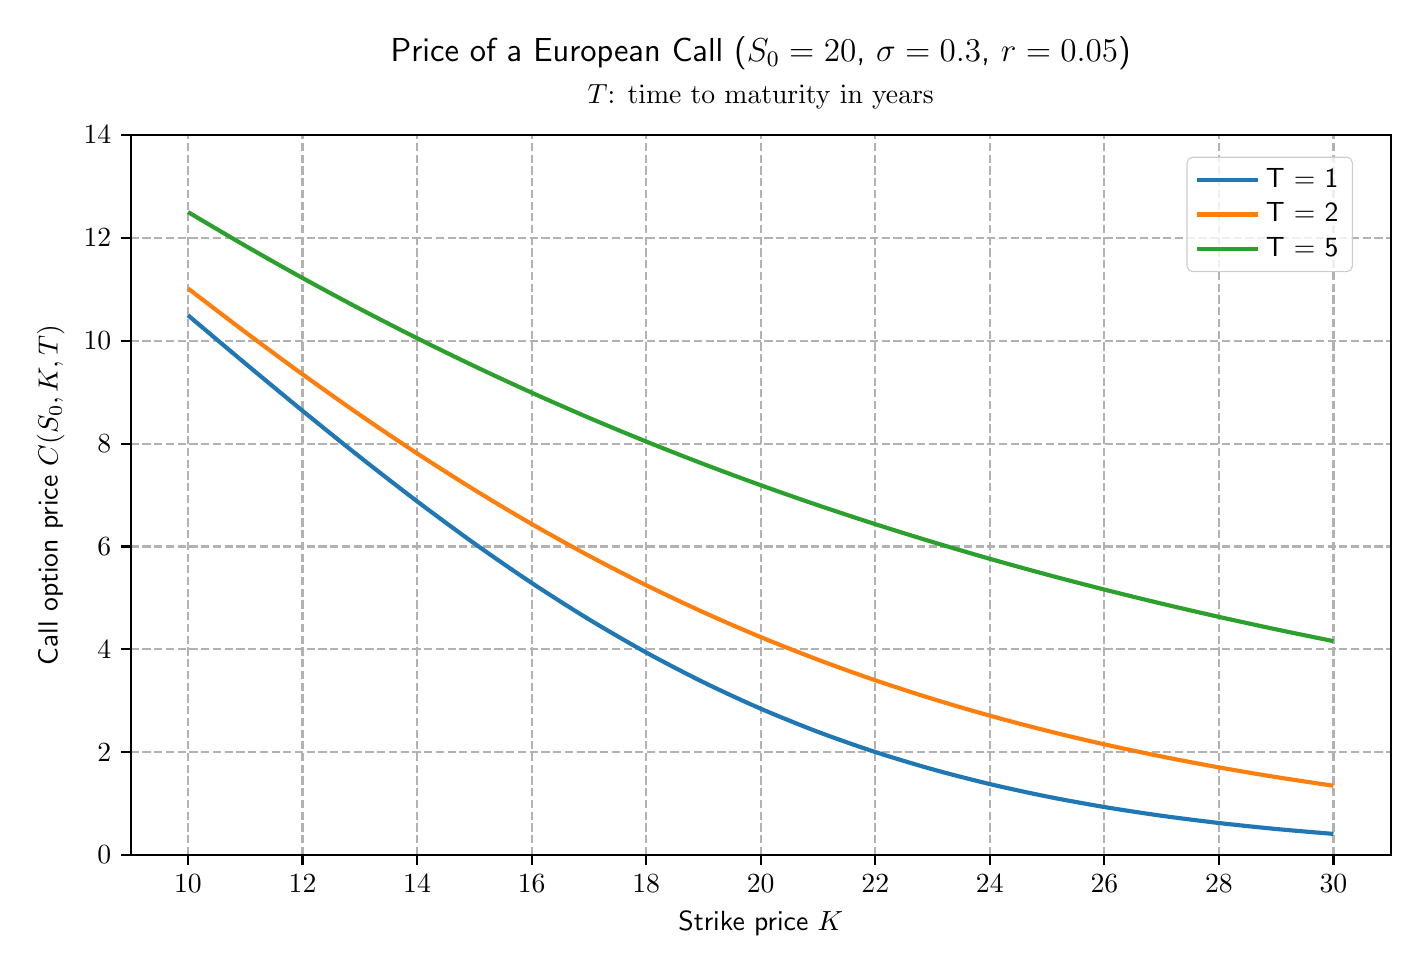
\begin{tikzpicture}
\begin{axis}[mpl, mplgrid, width=6.3in, height=3.6in, xmin=9, xmax=31, ymin=0, ymax=14,
  title style={align=center},
  title={\fontsize{12}{14}\selectfont\sffamily Price of a European Call ($S_0 = 20$, $\sigma = 0.3$, $r = 0.05$)\\[3pt] $T$: time to maturity in years},
  xlabel={\fontsize{10}{12}\selectfont\sffamily Strike price $K$}, ylabel={\fontsize{10}{12}\selectfont\sffamily Call option price $C(S_0,K,T)$},
  legend pos=north east, legend style={font=\fontsize{10}{12}\selectfont\sffamily}]
\addplot[tabblue, line width=1.5pt, smooth] coordinates {(10,10.4965) (11,9.5600) (12,8.6390) (13,7.7421) (14,6.8791) (15,6.0596) (16,5.2924) (17,4.5842) (18,3.9395) (19,3.3602) (20,2.8463) (21,2.3954) (22,2.0040) (23,1.6676) (24,1.3808) (25,1.1383) (26,0.9347) (27,0.7647) (28,0.6237) (29,0.5073) (30,0.4116)};
\addlegendentry{T = 1}
\addplot[taborange, line width=1.5pt, smooth] coordinates {(10,11.0187) (11,10.1698) (12,9.3485) (13,8.5606) (14,7.8107) (15,7.1025) (16,6.4386) (17,5.8203) (18,5.2480) (19,4.7213) (20,4.2387) (21,3.7987) (22,3.3990) (23,3.0373) (24,2.7107) (25,2.4169) (26,2.1530) (27,1.9166) (28,1.7051) (29,1.5163) (30,1.3478)};
\addlegendentry{T = 2}
\addplot[tabgreen, line width=1.5pt, smooth] coordinates {(10,12.5032) (11,11.8484) (12,11.2209) (13,10.6215) (14,10.0503) (15,9.5072) (16,8.9918) (17,8.5034) (18,8.0412) (19,7.6043) (20,7.1916) (21,6.8020) (22,6.4344) (23,6.0878) (24,5.7611) (25,5.4531) (26,5.1628) (27,4.8893) (28,4.6316) (29,4.3887) (30,4.1598)};
\addlegendentry{T = 5}
\end{axis}
\end{tikzpicture}}
\caption{Cell 44 with the new version of the pricer.}
\label{fig:call}
\end{figure}

\ansbox{The new \texttt{black\_scholes\_eur\_call(r, T, S0, sigma, K, return\_greeks=False)} returns the price, as cell 43 did, and with \texttt{return\_greeks=True} a dictionary with the price and the Greeks $\Delta,\Gamma,\mathcal V,\Theta,\rho$ of Theorem~2, \eqref{eq:callgreeks}. For $S_0=K=100$, $r=0.05$, $\sigma=0.2$, $T=1$:
\[
\begin{array}{cccccc}
c & \Delta & \Gamma & \mathcal V & \Theta & \rho\\ \midrule
10.450584 & 0.636831 & 0.018762 & 37.524035 & -6.414028 & 53.232482
\end{array}
\]}

% ============================================================================ HW 2/3
\bigskip
\begin{thmbox}{Put--call parity; Lesson 3, cell 30}
For a European call and a European put on the same non-dividend-paying stock, with the same strike $K$ and maturity $T$, at time $0$,
\begin{equation}\label{eq:parity}
c-p=S_0-K e^{-rT}.
\end{equation}
\end{thmbox}

\begin{lembox}{Black--Scholes--Merton price of a European put; from Theorems~1 and 3}
With $d_1,d_2$ as in \eqref{eq:d1d2},
\begin{equation}\label{eq:put}
p=K e^{-rT}N(-d_2)-S_0\,N(-d_1).
\end{equation}
\end{lembox}

\noindent\textit{Proof.} The standard normal density is symmetric, so $N(-x)=1-N(x)$ for every $x$. We solve \eqref{eq:parity} for $p$ and insert \eqref{eq:call}:
\begin{align*}
p &= c-S_0+Ke^{-rT} && \text{(Theorem~3, \eqref{eq:parity})}\\
&= S_0N(d_1)-Ke^{-rT}N(d_2)-S_0+Ke^{-rT} && \text{(Theorem~1, \eqref{eq:call})}\\
&= Ke^{-rT}\bigl(1-N(d_2)\bigr)-S_0\bigl(1-N(d_1)\bigr) && \text{(grouping)}\\
&= Ke^{-rT}N(-d_2)-S_0N(-d_1). && \text{($1-N(x)=N(-x)$)} \tag*{$\square$}
\end{align*}

\needspace{8\baselineskip}
\begin{exercise}{HW 2/3}
Implement the BSM pricer for European put option.
\end{exercise}
\solution
\subhead{New version.} The put pricer is the call pricer of cell 43 with three changes:
\begin{itemize}
\item \texttt{change \# 1}: the name \texttt{black\_scholes\_eur\_put} (same arguments);
\item \texttt{change \# 2}: $N(-d_1)$ and $N(-d_2)$ in place of $N(d_1)$ and $N(d_2)$;
\item \texttt{change \# 3}: the return line is the put price of Lemma~1, \eqref{eq:put} (with the argument \texttt{K}).
\end{itemize}
\par\smallskip\noindent\begin{minipage}{\linewidth}\begin{lstlisting}[style=prof,title={the put pricer}]
"""The pricing function of European put option"""
# change # 1
#Delete.    def black_scholes_eur_call(r: float, T: float, S0: float, sigma: float,
#Delete.                               K: Union[float, List[float], np.ndarray]) -> np.ndarray:
# replace by
def black_scholes_eur_put(r: float, T: float, S0: float, sigma: float,
                          K: Union[float, List[float], np.ndarray]) -> np.ndarray:
# end change # 1
    """
    Black-Scholes pricer of European put option on non-dividend-paying stock

    param r: risk-free interest rate (which is constant)
    param T: time to maturity (in years)
    param S0: initial spot price of the underlying stock
    param sigma: volatility of the underlying stock
    param K: strike price (or prices)
    """
    # check conditions
    assert sigma > 0

    K = np.array([K]) if isinstance(K, float) else np.array(K)

    d1_vec = ( np.log( S0 / K ) + ( r + 0.5 * sigma**2 ) * T ) / ( sigma * T**0.5 )
    d2_vec = d1_vec - sigma * T**0.5

    # change # 2
    #Delete.    N_d1_vec = norm.cdf(d1_vec)
    #Delete.    N_d2_vec = norm.cdf(d2_vec)
    # replace by
    N_minus_d1_vec = norm.cdf(-d1_vec)
    N_minus_d2_vec = norm.cdf(-d2_vec)
    # end change # 2

    # change # 3
    #Delete.    return N_d1_vec * S0 - K_vec * np.exp((-1.0)*r*T) * N_d2_vec
    # replace by
    return K * np.exp((-1.0)*r*T) * N_minus_d2_vec - S0 * N_minus_d1_vec
    # end change # 3
\end{lstlisting}\end{minipage}\par\smallskip

\subhead{Test.} The running example, and the plot of cell 44 for the put (Figure~\ref{fig:put}):
\par\smallskip\noindent\begin{minipage}{\linewidth}\begin{lstlisting}[style=py,title={test of the put pricer}]
# test 1: S0 = K = 100, r = 0.05, sigma = 0.2, T = 1
print(black_scholes_eur_put(r=0.05, T=1.0, S0=100.0, sigma=0.2, K=100.0))

# test 2: the plot of cell 44 for the put
K_vec = np.arange(10, 30, 0.01)
T_vec = [1.0, 2.0, 5.0]

plt.figure(figsize=(10, 6))
for T in T_vec:
    plt.plot(K_vec, black_scholes_eur_put(r=0.05, T=T, S0=20.0, sigma=0.3, K=K_vec),
             label=f"T = {int(T)}")
plt.title('Price of a European Put ($S_0 = 20$, $\\sigma = 0.3$, $r = 0.05$)')
plt.xlabel('Strike price $K$')
plt.ylabel('Put option price $P(S_0,K,T)$')
plt.legend()
plt.grid(True)
plt.show()
\end{lstlisting}
\begin{lstlisting}[style=out,title={output}]
[5.57352602]
\end{lstlisting}\end{minipage}\par\smallskip
By hand, with $d_1=0.35$, $d_2=0.15$ of HW 2/2, \eqref{eq:put} gives
\begin{align*}
p &= 100\,e^{-0.05}N(-0.15)-100\,N(-0.35)\\
&\approx 41.89046-36.31694\\
&\approx 5.5735. && \checkmark
\end{align*}

\begin{figure}[!ht]
\centering
\resizebox{0.7\textwidth}{!}{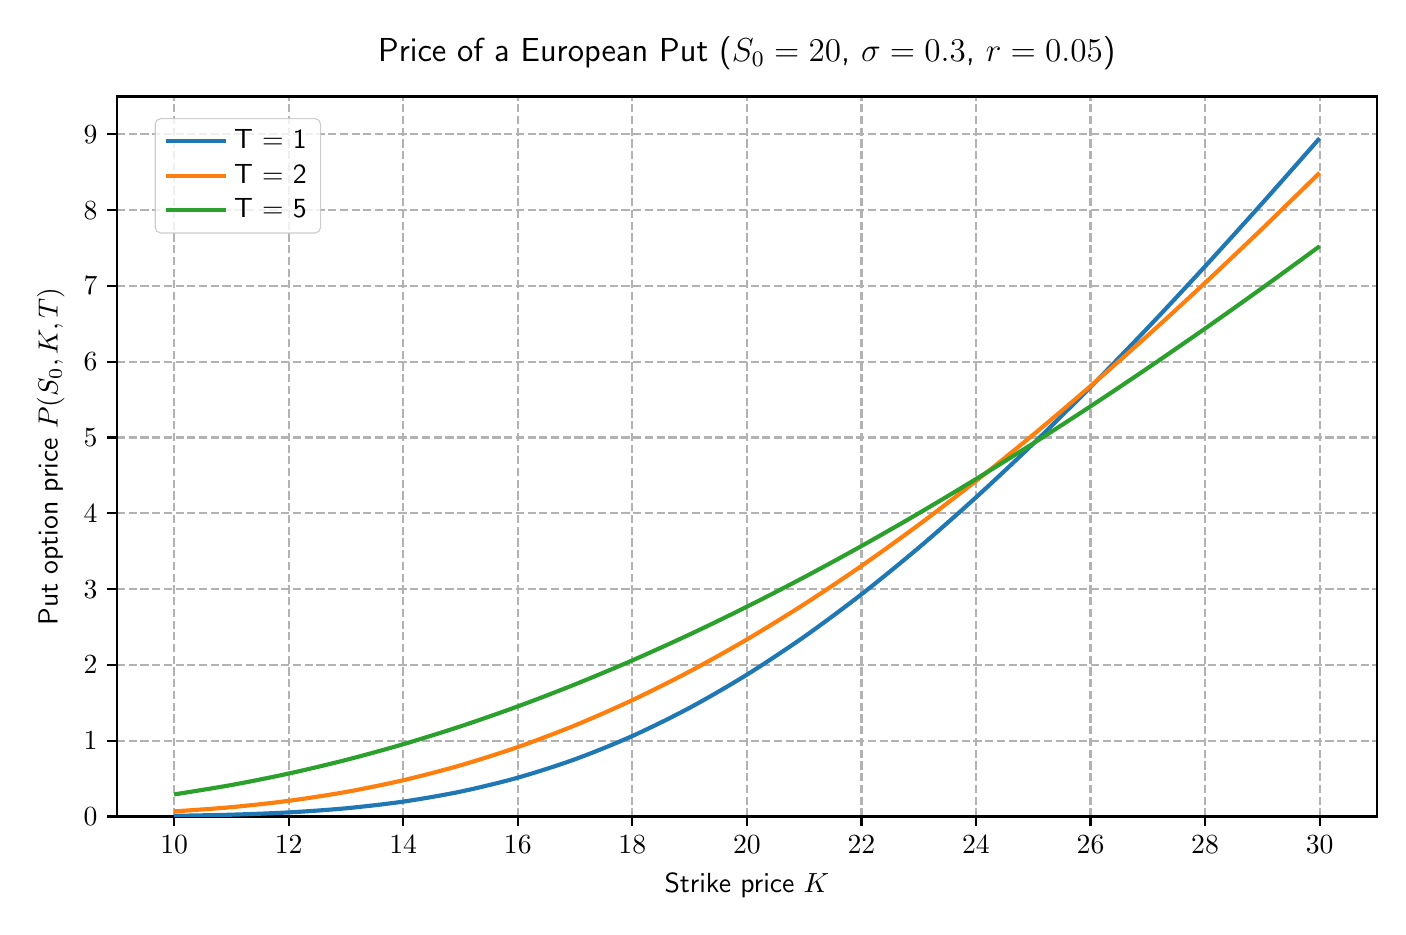
\begin{tikzpicture}
\begin{axis}[mpl, mplgrid, width=6.3in, height=3.6in, xmin=9, xmax=31, ymin=0, ymax=9.5,
  title style={align=center},
  title={\fontsize{12}{14}\selectfont\sffamily Price of a European Put ($S_0 = 20$, $\sigma = 0.3$, $r = 0.05$)},
  xlabel={\fontsize{10}{12}\selectfont\sffamily Strike price $K$}, ylabel={\fontsize{10}{12}\selectfont\sffamily Put option price $P(S_0,K,T)$},
  legend pos=north west, legend style={font=\fontsize{10}{12}\selectfont\sffamily}]
\addplot[tabblue, line width=1.5pt, smooth] coordinates {(10,0.0088) (11,0.0236) (12,0.0538) (13,0.1081) (14,0.1963) (15,0.3281) (16,0.5121) (17,0.7551) (18,1.0616) (19,1.4336) (20,1.8708) (21,2.3712) (22,2.9311) (23,3.5458) (24,4.2103) (25,4.9190) (26,5.6666) (27,6.4479) (28,7.2582) (29,8.0930) (30,8.9485)};
\addlegendentry{T = 1}
\addplot[taborange, line width=1.5pt, smooth] coordinates {(10,0.0671) (11,0.1230) (12,0.2066) (13,0.3235) (14,0.4784) (15,0.6751) (16,0.9160) (17,1.2025) (18,1.5351) (19,1.9132) (20,2.3355) (21,2.8003) (22,3.3055) (23,3.8485) (24,4.4268) (25,5.0378) (26,5.6788) (27,6.3472) (28,7.0406) (29,7.7566) (30,8.4930)};
\addlegendentry{T = 2}
\addplot[tabgreen, line width=1.5pt, smooth] coordinates {(10,0.2912) (11,0.4152) (12,0.5665) (13,0.7459) (14,0.9535) (15,1.1892) (16,1.4526) (17,1.7430) (18,2.0596) (19,2.4015) (20,2.7676) (21,3.1568) (22,3.5680) (23,4.0002) (24,4.4523) (25,4.9231) (26,5.4116) (27,5.9169) (28,6.4380) (29,6.9739) (30,7.5238)};
\addlegendentry{T = 5}
\end{axis}
\end{tikzpicture}}
\caption{Output of the test: put price against the strike.}
\label{fig:put}
\end{figure}

\ansbox{The function \texttt{black\_scholes\_eur\_put(r, T, S0, sigma, K)} returns the put price of Lemma~1, \eqref{eq:put},
\[
p=Ke^{-rT}N(-d_2)-S_0\,N(-d_1).
\]
For $S_0=K=100$, $r=0.05$, $\sigma=0.2$, $T=1$: $p\approx5.573526$.}

% ============================================================================ HW 2/4
\needspace{8\baselineskip}
\begin{exercise}{HW 2/4}
With the call and put pricer, check if Put-Call parity holds in practice.
\end{exercise}
\solution
\subhead{What is checked.} We compute both sides of Theorem~3, \eqref{eq:parity}: the left side $c-p$ with the two pricers, the right side $S_0-Ke^{-rT}$ directly, for the strikes and maturities of cell 44 ($2000$ strikes from $10$ to $30$, $T=1,2,5$, $S_0=20$, $\sigma=0.3$, $r=0.05$).
\par\smallskip\noindent\begin{minipage}{\linewidth}\begin{lstlisting}[style=prof,title={parity check}]
# put-call parity at t = 0:  c - p = S0 - K e^{-rT}
K_vec = np.arange(10, 30, 0.01)
T_vec = [1.0, 2.0, 5.0]
S0, sigma, r = 20.0, 0.3, 0.05

plt.figure(figsize=(10, 6))
for T in T_vec:
    c = black_scholes_eur_call(r=r, T=T, S0=S0, sigma=sigma, K=K_vec)
    p = black_scholes_eur_put(r=r, T=T, S0=S0, sigma=sigma, K=K_vec)
    left = c - p                              # from the pricers
    right = S0 - K_vec * np.exp(-r * T)       # from the parity formula
    print(f"T = {int(T)}:  max |(c - p) - (S0 - K e^(-rT))| = {np.max(np.abs(left - right)):.1e}")
    plt.plot(K_vec, left, label=f"c - p,  T = {int(T)}")
    plt.plot(K_vec, right, 'k--', linewidth=0.8)
plt.title('Put-call parity: $c - p$ (colour) and $S_0 - Ke^{-rT}$ (black dashed)')
plt.xlabel('Strike price $K$')
plt.ylabel('value')
plt.legend()
plt.grid(True)
plt.show()
\end{lstlisting}
\begin{lstlisting}[style=out,title={output}]
T = 1:  max |(c - p) - (S0 - K e^(-rT))| = 5.3e-15
T = 2:  max |(c - p) - (S0 - K e^(-rT))| = 5.3e-15
T = 5:  max |(c - p) - (S0 - K e^(-rT))| = 4.4e-15
\end{lstlisting}\end{minipage}\par\smallskip

\begin{figure}[!ht]
\centering
\resizebox{0.7\textwidth}{!}{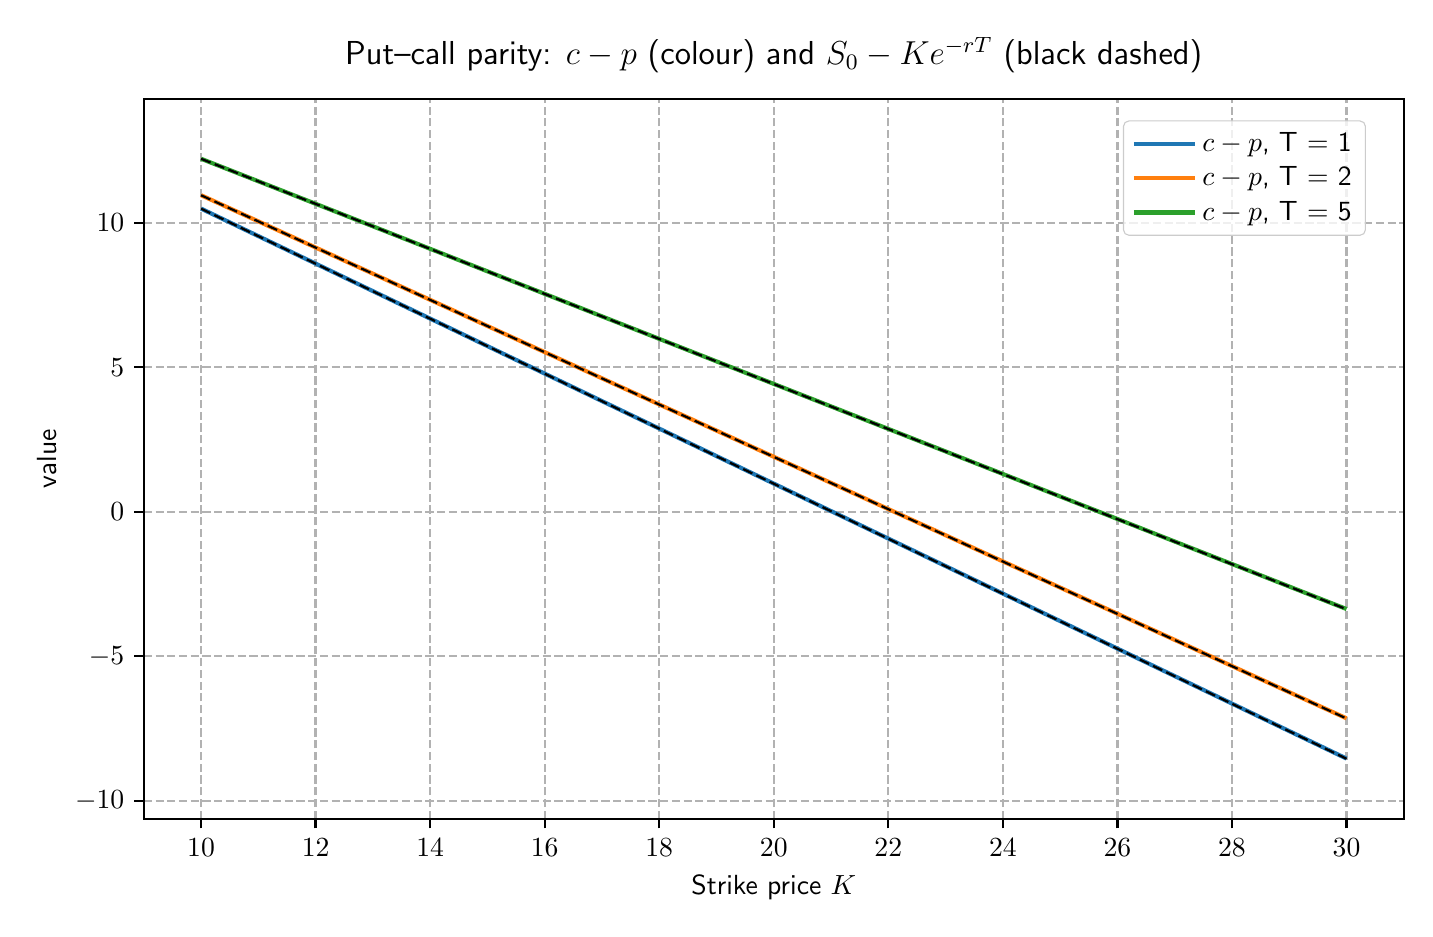
\begin{tikzpicture}
\begin{axis}[mpl, mplgrid, width=6.3in, height=3.6in, xmin=9, xmax=31,
  title={\fontsize{12}{14}\selectfont\sffamily Put\textendash call parity: $c - p$ (colour) and $S_0 - Ke^{-rT}$ (black dashed)},
  xlabel={\fontsize{10}{12}\selectfont\sffamily Strike price $K$}, ylabel={\fontsize{10}{12}\selectfont\sffamily value},
  legend pos=north east, legend style={font=\fontsize{10}{12}\selectfont\sffamily}]
\addplot[tabblue, line width=1.5pt] coordinates {(10,10.4877) (12,8.5852) (14,6.6828) (16,4.7803) (18,2.8779) (20,0.9754) (22,-0.9270) (24,-2.8295) (26,-4.7320) (28,-6.6344) (30,-8.5369)};
\addlegendentry{$c-p$,  T = 1}
\addplot[black, line width=0.8pt, mpldash, domain=10:30, samples=2, forget plot] {20 - x*exp(-0.05*1)};
\addplot[taborange, line width=1.5pt] coordinates {(10,10.9516) (12,9.1420) (14,7.3323) (16,5.5226) (18,3.7129) (20,1.9033) (22,0.0936) (24,-1.7161) (26,-3.5258) (28,-5.3354) (30,-7.1451)};
\addlegendentry{$c-p$,  T = 2}
\addplot[black, line width=0.8pt, mpldash, domain=10:30, samples=2, forget plot] {20 - x*exp(-0.05*2)};
\addplot[tabgreen, line width=1.5pt] coordinates {(10,12.2120) (12,10.6544) (14,9.0968) (16,7.5392) (18,5.9816) (20,4.4240) (22,2.8664) (24,1.3088) (26,-0.2488) (28,-1.8064) (30,-3.3640)};
\addlegendentry{$c-p$,  T = 5}
\addplot[black, line width=0.8pt, mpldash, domain=10:30, samples=2, forget plot] {20 - x*exp(-0.05*5)};
\end{axis}
\end{tikzpicture}}
\caption{Output of the parity check: the coloured curves $c-p$ from the pricers lie on the dashed lines $S_0-Ke^{-rT}$.}
\label{fig:parity}
\end{figure}

\subhead{Why the difference is so small.} By \eqref{eq:call}, \eqref{eq:put} and $N(x)+N(-x)=1$,
\begin{align*}
c-p &= S_0N(d_1)-Ke^{-rT}N(d_2)-Ke^{-rT}N(-d_2)+S_0N(-d_1)\\
&= S_0\bigl(N(d_1)+N(-d_1)\bigr)-Ke^{-rT}\bigl(N(d_2)+N(-d_2)\bigr)\\
&= S_0-Ke^{-rT}.
\end{align*}
So the two sides are equal exactly, and the difference of order $10^{-15}$ printed above is only the rounding error of the computer (about $10^{-16}$ relative to numbers of size $S_0=20$).

\emph{Comment.} In real markets parity holds only approximately: there are bid--ask spreads and trading costs, many stocks pay dividends and many options are American, and Theorem~3 assumes none of these. For the pricers it holds because the call and the put are priced with the same $\sigma$; pricing them with different volatilities would break it.

\ansbox{Yes. For all $3\times2000$ contracts of cell 44, our pricers satisfy put--call parity, Theorem~3, \eqref{eq:parity},
\[
c-p=S_0-Ke^{-rT},
\]
up to a difference of at most $5.3\cdot10^{-15}$, which is floating-point rounding: for the BSM formulas the two sides are equal exactly.}

\end{document}
